\chapter{血液净化与肾脏替代治疗}

\section{前沿学术综述}

血液净化治疗起源于血液透析,伴随机械和电子技术的进展,血液净化治疗方式也逐渐拓展,应用范围不断扩大。临床上将利用净化装置通过体外循环方式清除体内代谢产物、异常血浆成分以及蓄积在体内的药物或毒物,以纠正机体内环境紊乱的一组治疗技术,统称为血液净化或肾脏替代治疗(renal
replacement therapy,RRT)技术。

根据血液净化方式不同可分为:血液透析、血液滤过、血液灌流、血浆置换、免疫吸附等。腹膜透析虽然没有经过体外循环,但从广义上讲,也应属于在血液净化疗法之内。根据血液净化时间不同可分为:间断血液净化和连续性肾脏替代治疗(continuous
renal replacement therapy,CRRT)。

血液净化治疗不仅广泛应用于急性肾衰竭(acute renal
failure)合并心血管功能不全、脑水肿、高分解代谢状态、严重的全身水肿等,而且,目前临床已广泛用于治疗重症感染、ARDS、急性重症胰腺炎等非肾脏疾病。但血液净化的治疗效果受临床实施的多种因素影响,包括治疗的时机、剂量及模式等,目前并没有统一的肾脏替代治疗标准,不同的疾病状态需采用个体化的治疗策略。

\subsubsection{肾脏替代治疗的治疗时机}

在合适的时机开始肾脏替代治疗,能够更好地发挥其调节容量、纠正酸碱及电解质紊乱、改善氮质血症等优势。目前临床肾脏替代治疗时机的定义仍多参考危险、损伤、衰竭、丧失终末期肾脏疾病评分、急性肾损伤网络标准,根据血尿素氮、肌酐及尿量进行判断。近期的研究
\protect\hyperlink{text00018.htmlux5cux23ch1-17}{\textsuperscript{{[}1{]}}}
\textsuperscript{,}
\protect\hyperlink{text00018.htmlux5cux23ch2-17}{\textsuperscript{{[}2{]}}}
也在探讨人中性粒细胞明胶酶相关脂质运载蛋白(NGAL)、胱蛋白酶抑制剂C(CyC)、N-乙酰-β-D氨基葡糖苷酶(NAG)、肾损伤分子-1(KIM-1)、α1微球蛋白等生物学标记物与肾脏替代治疗的相关性,但目前肾损伤相关生物学标记物在连续肾脏替代治疗时机选择中的作用的相关研究结论不完全一致,仍未能有效地用于临床连续肾脏替代治疗时机的判定。

在急性肾损伤(acute kidney injury,AKI)患者中,Carl等
\protect\hyperlink{text00018.htmlux5cux23ch3-17}{\textsuperscript{{[}3{]}}}
对130例急性肾损伤合并重症感染的患者按照尿素氮水平是否大于100mg/dl行肾脏替代治疗,结果表明早期行肾脏替代治疗(平均尿素氮66mg/dl)比晚期治疗(平均尿素氮137mg/dl)能够明显降低患者的14天、28天、365天的病死率。新近的Meta分析纳入15项研究
\protect\hyperlink{text00018.htmlux5cux23ch4-17}{\textsuperscript{{[}4{]}}}
,结果表明在伴有急性肾损伤的重症患者中,与晚期肾脏替代治疗相比,早期肾脏替代治疗组或者28天病死率显著降低。由此可见,对需行肾脏替代治疗的急性肾损伤患者,早期开始肾脏替代治疗可能可以更有效改善患者预后。

但并非所有合并急性肾损伤的重症患者均能从肾脏替代治疗中获益。不加选择开始肾脏替代治疗可能并不能达到理想的治疗效果。Elseviers等
\protect\hyperlink{text00018.htmlux5cux23ch5-17}{\textsuperscript{{[}5{]}}}
研究发现,在1303例合并急性肾损伤的重症患者中,行连续肾脏替代治疗患者比采用常规治疗组(无连续肾脏替代治疗)的病死率更高,经过病情严重程度校正、不同疾病亚组分析,结果仍表明连续肾脏替代治疗是重症急性肾损伤患者病死率的独立危险因素。提示合并急性肾损伤重症患者的临床治疗中需慎重把握实施肾脏替代治疗的时机。此外,在慢性肾衰竭患者过早地进行连续肾脏替代治疗或维持性血液透析治疗,可能并不能减轻患者病情,且造成医疗资源浪费、增加患者及社会经济负担。

可见,对肾脏替代治疗指征把握及首次开始时机目前仍缺乏统一的标准。目前推荐在急性肾损伤患者出现明显的并发症前,尽早开始肾脏替代治疗,血尿素氮、尿量等指标可以作为开始肾脏替代治疗的参考,但尚缺乏统一的、理想的血清学标准或临床标准,仍需要进一步研究探索。

\subsubsection{肾脏替代治疗的治疗剂量}

肾脏替代治疗主要通过对体内溶质及溶剂的清除发挥其治疗作用,因此肾脏替代治疗的治疗剂量即溶质和溶剂的清除剂量对其治疗效果会产生直接的影响。过低的治疗剂量可能导致肾脏替代治疗效果不佳,延误病情;而剂量设置过大一方面可能造成体内有益物质丢失过多,另一方面也明显增加临床工作量和治疗费用。因此,临床治疗中需根据患者病情需要设置合适的肾脏替代治疗治疗剂量。

近年来的研究不断探讨合并急性肾损伤的重症患者肾脏替代治疗的合适治疗剂量。近期两项大规模研究,即ATN
\protect\hyperlink{text00018.htmlux5cux23ch6-17}{\textsuperscript{{[}6{]}}}
和RENAL
\protect\hyperlink{text00018.htmlux5cux23ch7-17}{\textsuperscript{{[}7{]}}}
的研究结果均显示较大剂量肾脏替代治疗与常规剂量相比(ATN:每小时35ml/kg对比每小时20ml/kg;RENAL:每小时40ml/kg对比每小时25ml/kg),并不能改善急性肾损伤患者的预后。最近的一项纳入12项研究、3999例患者的Meta分析
\protect\hyperlink{text00018.htmlux5cux23ch8-17}{\textsuperscript{{[}8{]}}}
结果也表明,无论是在所有的急性肾损伤患者,还是在重症感染患者中,高剂量肾脏替代治疗组(≥每小时30ml/kg)与低剂量肾脏替代治疗组(<每小时30ml/kg)患者的病死率无统计学差异。基于既往的研究,目前认为每小时20~45ml/kg范围内的肾脏替代治疗治疗剂量对急性肾损伤患者的预后并无明显影响。

通过清除炎症因子、调节内环境等机制,肾脏替代治疗在重症感染及感染性休克的治疗中发挥重要作用。既往观点认为,在重症感染及感染性休克患者中,需要高流量血液滤过,可能更有效地清除炎症因子,改善患者预后,因此一般建议每小时35ml/kg以上的超滤率,但理想的重症感染肾脏替代治疗剂量仍在进一步探索。Zhang等
\protect\hyperlink{text00018.htmlux5cux23ch9-17}{\textsuperscript{{[}9{]}}}
在重症感染合并急性肾损伤的患者中采用每小时50ml/kg及85ml/kg超滤率进行肾脏替代治疗,结果发现两组患者的28、90天病死率均无明显差异。已完成的IVORIE研究(结果尚未正式发表)同样提示每小时70ml/kg的治疗剂量并不能比35ml/kg改善感染性休克合并急性肾损伤患者预后,且患者血管活性药物需求量、氧合及住院时间等两组间均无显著差异,而高剂量治疗组患者的血磷、维生素C等丢失更多。因此,目前尚无明确证据更高的肾脏替代治疗治疗剂量能更有效,现仍建议在重症感染及感染性休克患者中选择每小时35~45ml/kg的剂量,更高的治疗剂量并不常规推荐。

在其他疾病的治疗中,肾脏替代治疗治疗剂量需根据临床实际的治疗目标决定。对于横纹肌溶解患者,由于肌肉破坏释放大量肌红蛋白,可能进一步导致急性肾功能损害,行肾脏替代治疗的目标在于清除血液内肌红蛋白,此时应选择高流量血液滤过,应选择较高的治疗剂量,并根据监测的血肌红蛋白、肌酸激酶及肾功能情况进行调整;在常规治疗无效的心衰患者中,肾脏替代治疗为调节容量,此时可采用缓慢持续超滤等模式,设置较低的治疗剂量进行缓慢容量调整。一般认为,心力衰竭患者行肾脏替代治疗的超滤速度≤500ml/每小时,血流速≤40ml/分,持续的时间应在8小时以上。此外,在严重电解质紊乱、高热、中毒等其他非肾性肾脏替代治疗适用患者中,也均需根据肾脏替代治疗的作用、临床需要调整的目标及速度确定最终的肾脏替代治疗治疗剂量,并动态评估患者的病情变化,对肾脏替代治疗的治疗剂量也进行动态调整。

\subsubsection{肾脏替代治疗的治疗模式}

肾脏替代治疗有缓慢持续超滤、持续静脉-静脉血液滤过、持续静脉-静脉血液透析、血液灌流等多种模式,不同模式治疗疾病的机制并不相同,因此应根据治疗目的,选择合适的肾脏替代治疗模式。此外,选择持续模式或间断模式(intermittent
renal replacement
therapy,IRRT)方面,对不同的疾病人群,适用的范围也并不一致。

应根据患者的疾病类型及治疗目标选择不同的连续肾脏替代治疗治疗模式。在急性肾损伤或慢性肾衰竭患者中,若仅需改善氮质血症、纠正酸碱及电解质紊乱,由于清除的均为中小分子物质,选择血液透析效率更高,疗效更确切。在重症感染、急性胰腺炎或横纹肌溶解患者中,为清除炎症因子、肌红蛋白等中大分子量溶质,应选择血液滤过模式,同时配合合适的治疗剂量。而在肾衰竭合并水负荷过重或顽固性心衰需调节容量的患者,连续肾脏替代治疗选择超滤模式可以达到清除体内过多水分的治疗目标。处理中毒的患者时,根据毒物的性质不同,可以选择血液灌流、血浆置换等模式进行治疗。在重症患者的处理中,由于病情较复杂,也常常需要进行多种模式连续肾脏替代治疗的联合,如血液滤过联合血液透析、血液灌流联合血液透析等。

在肾脏替代治疗持续的时间选择方面,亦即采用持续或间断的模式,临床也一直在探讨。近期的大量研究结果表明,在采用连续肾脏替代治疗和间歇肾脏替代治疗的患者中,患者病死率、重症医学科住院时间、肾功能恢复情况等均无明显差异。连续肾脏替代治疗较间歇肾脏替代治疗能更好地维持血流动力学稳定、减少血管活性药物的应用,更有效地调节水及电解质的稳定,但同时也会带来营养物质丢失增多、感染几率增加、花费较高等不良影响,因此目前并不推荐所有需行肾脏替代治疗的患者均采用连续肾脏替代治疗模式
\protect\hyperlink{text00018.htmlux5cux23ch9-17}{\textsuperscript{{[}9{]}}}
。此外,亦有学者采用持续低效透析(sustained low-efficiency
dialysis,SLED)治疗急性肾衰竭,发现持续低效透析既具备连续肾脏替代治疗缓慢持续、对患者血流动力学影响小的优势,也易于操作、减少了治疗费用,并且能够改善患者的预后,可能是介于连续肾脏替代治疗与间歇肾脏替代治疗之间的一种选择
\protect\hyperlink{text00018.htmlux5cux23ch10-17}{\textsuperscript{{[}10{]}}}
。

随着认识的深入和技术的进步,也逐渐出现新的肾脏替代治疗治疗模式,如近年来的研究证实多黏菌素B血液灌流能够降低重症感染患者的血清内毒素水平、降低患者病死率。分子吸附再循环系统(molecular
adsorbents recycling system,MARS)、持续性血浆滤过吸附(continuous
plasma filtration
adsorption,CPFA)也逐步应用于临床,被证实可能改善患者的预后。但相关的研究病例数较少及研究人群的异质性等因素,对于一些新治疗模式的疗效仍存在争议,仍需要进一步的临床研究。

\section{临床问题}

\subsection{血液滤过的基本原理与实施}

\subsubsection{何谓血液滤过?}

自从1967年,Henderson等开始研究血液滤过,并逐步应用于临床,1977年联邦德国医生Kramer首次将连续动-静脉血液滤过(continuous
arterio-venous
hemofiltration,CAVH)用于治疗急性肾衰竭合并水潴留患者。近10多年来,随着认识的逐步深入,血液滤过在危重患者中得到了越来越广泛的应用。

血液滤过是血液通过滤器时,大部分体内的水分、电解质、中小分子物质通过滤过膜被除去,然后补充相似体积的与细胞外液成分相似的电解质溶液(称置换液),从而达到排出体内废物和过多水分的目的。

近年来为提高疗效,满足不同病情需要又衍生出多种改良型血液滤过系列。

(1)连续动-静脉血液滤过 指将动脉血液引入一小型、高效、低阻滤器,依靠人体自身动-静脉压力差作为循环动力,清除体内潴留水分及部分代谢产物,并将已经净化的血液经静脉输回体内,这一连续不断进行的血液净化过程为连续动-静脉血液滤过。其工作原理为超滤,是通过滤器膜两侧压力差来清除水分和部分溶质的。

(2)连续动-静脉血液滤过透析(continuous arterio-venous
hemodiafiltration,CAVHD) 由于连续动-静脉血液滤过对小分子尿毒物质的清除较差,清除氮质代谢产物不多,故在此基础上又发展出连续动-静脉血液滤过透析。连续动-静脉血液滤过透析是在连续动-静脉血液滤过的基础上实施的超滤和透析,它通过滤器膜两侧的压力差及浓度梯度达到清除水分和溶质的目的,从而可以清除过多的水分,又能清除一定的氮质代谢产物,保持机体内环境的稳定。

(3)连续静脉-静脉血液滤过(continuous veno-venous
hemofiltration,CVVH) 是在连续动脉-静脉血液滤过原理的基础上借助单针双腔管建立单静脉通道,外加血泵驱动血液维持一定的血流量而建立起来的一种持续性血液滤过疗法,它简化了连续动脉-静脉血液滤过的技术,明显减少了血管通路上的并发症。连续静脉-静脉血液滤过使用血泵可使血流量达到80~250ml/分。

(4)连续静脉-静脉血液滤过透析(continuous veno-venous
hemodiafiltration,CVVHD) 原理基本与连续动-静脉血液滤过透析相同,但血管通路的建立则与连续静脉-静脉血液滤过一样,其可避免动静脉短路引起的血液分流,不仅可以更完善地清除患者体内过多的水分和氮质代谢产物,而且还可以使血管通路的并发症明显减少。

\subsubsection{血液滤过的主要原理是什么?}

血液滤过是模拟正常肾小球的滤过作用原理,以对流为基础的血液净化技术。血循环用或不用血泵,将血液通过高通透性膜制成的滤器,跨膜压由患者的平均动脉压加滤液侧负压,驱使水分经滤过膜进入滤液,溶质以等渗性对流转运和水一起穿过透析膜。再通过输液装置,在滤器前或后,补充与细胞外液成分相似的电解质溶液(置换液)以防容量缺失,达到血液净化目的。

溶质的传递方式基本上有两大类形式,即弥散和对流,血液滤过主要是模拟正常肾小球的滤过功能,即主要是通过对流的方式来清除水与溶质的。这与血液透析的溶质传递方式不同,血液透析主要是通过弥散作用来清除溶质。由于血液滤过滤器的通透性较高,不同分子量物质的清除率基本相似。而血液透析的清除率与分子量的大小成反比,与膜的筛系数无明显关系。血液滤过对中分子物质的清除优于血液透析。而血液透析对于小分子物质的清除较好。

血滤器一般由高通透性的聚矾膜、聚丙烯膜、聚丙烯酸甲脂组成,超滤率>30ml/kPa·h\textsuperscript{-1}
·m\textsuperscript{-2}
。在连续静脉-静脉血液滤过时的溶质清除(CL)的计算法为:CL=超滤率(QF)×筛系数(Sc)。超滤液中溶质(含尿素)浓度与血浆相近,即Sc=1。因此,如QF平均为10ml/分,尿素清除率也为10ml/分。

\subsubsection{血液滤过时影响水和溶质清除的主要因素有哪些?}

血液滤过时影响水和溶质清除的因素如下。

(1)滤器性能及流体力学特征 滤器性能首先取决于膜材料,但与滤器长短、口径、几何图形也有关。刚性管道两端的压力降=血液黏度×n×血流量/(π×管道半径\textsuperscript{4}
)。连续动脉-静脉血液滤过时,动脉压为驱动力。当动脉压较低时,减少管道与滤器阻力对维持有效超滤至关重要。选择一个粗口径、短血路和中空纤维内径较粗的短滤器,可产生一个低阻力、高血流量。12.5cm的滤器较20cm的滤器阻力下降40%~60%,即使在低血压时仍能超滤。

(2)滤器内压力梯度 滤器内静水压与血液侧压及滤液侧负压液共同影响超滤。可调控部分是滤液收集器与滤器之间的距离,为高度差每增加1cm产生0.09kPa(0.7mmHg)负压,通常滤液收集器低于床边20~40cm,必要时加用吸引器或负压泵来调节。目前许多血滤机再滤液侧装有可调节正压或负压的泵,来调节滤器内外的压力梯度。滤器内胶体渗透压与血浆蛋白有关。

(3)血液黏滞度、血流量与超滤 若血细胞比容>0.45,则超滤率降低,血流量在90~250ml/分时,血流量与超滤率明显相关。

\subsubsection{血液滤过的适应证有哪些?}

血液滤过的适应证主要包括:

(1)高血容量性心功能不全、急性肺水肿。

(2)严重酸碱及电解质紊乱:①代谢性酸中毒;②代谢性碱中毒;③高钠或低钠血症;④高钾血症。

(3)药物中毒,尤其是多种药物的复合中毒。

(4)急、慢性肾衰竭有以下情况时:①低血压或血液透析时循环不稳定;②血流动力学不稳定;③需要实施全静脉营养;④伴有多器官功能衰竭。

(5)尿毒症性心包炎、皮肤瘙痒、周围神经病变等。病变与中分子毒素有关,可采用血液滤过清除中分子毒素。

(6)肝性脑病、肝肾综合征。

(7)感染性休克。

(8)ARDS。

(9)多器官功能衰竭

\subsubsection{血液滤过的常见并发症有哪些?}

(1)导管相关的并发症 穿刺部位出血、血肿;穿刺引起气胸、血气胸;导管相关感染;导管异位。

(2)血液滤过器及管道相关的并发症 滤器内漏血,与滤器中空纤维中压力过高有关;滤器和管道内血栓堵塞,与血滤管路扭曲、导管贴壁或未应用肝素抗凝有关:泵管破裂,与泵管使用时间过长有关。

(3)与抗凝相关的并发症 肝素用量过大引起全身多个部位出血;滤器内凝血;血小板降低。

(4)全身并发症 超滤液过多,置换液补充不足,导致血容量不足和低血压;补液不当引起酸碱平衡失调及电解质紊乱;长期血液滤过的患者还应注意激素丢失引起的内分泌系统紊乱。

\subsubsection{与间断血液透析及腹膜透析比较,连续肾脏替代治疗有何优点?}

在重症患者治疗中,与间断血液透析及腹膜透析治疗比较(表\ref{tab12-1}),持续血液滤过等连续肾脏替代治疗措施在治疗急性肾衰、多器官功能衰竭中有突出的优点。

\begin{table}[htbp]
\centering
\caption{连续肾脏替代治疗与血液透析、腹膜透析的比较}
\label{tab12-1}
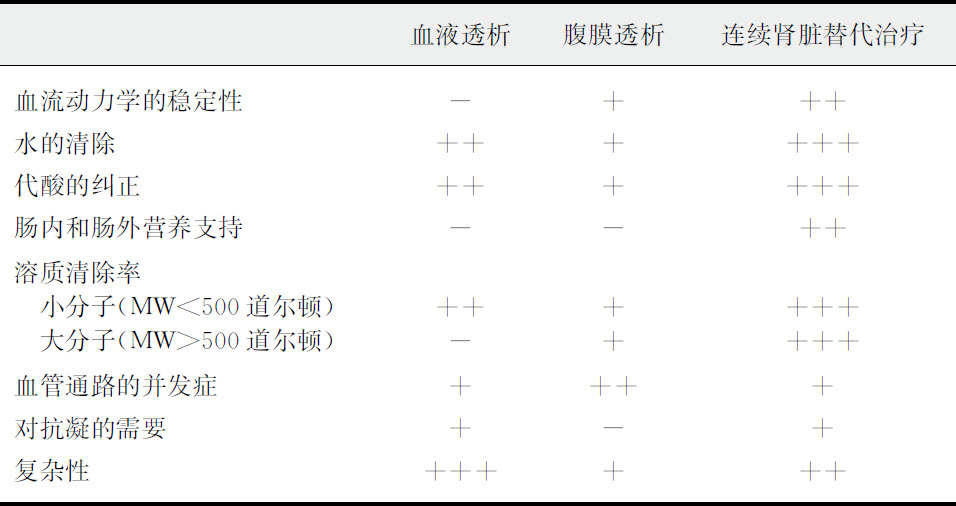
\includegraphics{./images/Image00093.jpg}
\end{table}

\subsubsection{与间断血液透析比较,为什么实施连续肾脏替代治疗时血液动力学更稳定?}

间歇性血液透析和连续肾脏替代治疗临床上的主要差别是对危重患者的血液动力学影响。间歇性血液透析治疗容易导致危重患者血压降低,主要原因包括:

(1)血液透析迅速清除水和溶质,使血容量迅速降低,但交感神经缺乏正常反应。

(2)透析器生物相容性差,导致粒细胞激活和细胞因子释放。

(3)溶质和水分,特别是小分子溶质被迅速清除,导致细胞外液的晶体渗透压迅速降低,细胞外液向细胞内移动,结果导致细胞外液,特别是血管内容量的降低。

(4)血液透析的体外血流速度较快,对循环影响较大。原有严重心功能不全、休克或严重低氧血症患者不能耐受间歇性血液透析,甚至加重病情。

Mauritz报道的一项回顾性研究显示,163例腹腔感染的急性肾衰竭患者接受血液透析治疗时,透析期间有31.9%(52例)的患者发生严重的低血压。为纠正低血压而大量输液,结果透析后的容量负荷比透析前还高。由此可见,对于血流动力学不甚稳定的危重患者,采用血液透析治疗是不合适的。

应用连续肾脏替代治疗时,危重患者的血流动力学相对比较稳定,主要与以下因素有关:①血液滤过为持续性超滤,对水和溶质的清除速度较慢,对血容量影响较小;②细胞外液晶体渗透压降低较缓,细胞外液容量变化也较小;③血滤器的生物相容性较好;④血液滤过的体外血流速度较慢,对患者循环影响较小。可见,连续肾脏替代治疗对危重患者循环的干扰较小,更适合于血流动力学不甚稳定的危重患者。

\subsubsection{连续肾脏替代治疗与间断血液透析对中分子物质的清除效率有何不同?}

血液透析所采用的透析器膜的孔径较小,1000~2000道尔顿以下的溶质分子能够自由通透,而且血液透析是通过弥散的原理清除溶质,因此,血液透析几乎无法清除中分子物质。

连续肾脏替代治疗的滤器膜通透性较高,一般低于4万~5万道尔顿的溶质可被滤出。连续肾脏替代治疗主要通过对流清除溶质,对中分子量物质清除明显高于弥散的清除效率。

近年来非常重视β\textsubscript{2}
微球蛋白的清除,它不但可以导致淀粉样变等骨关节病变,还可用血浆β\textsubscript{2}
微球蛋白水平评价透析的充分性。使用高通量膜进行连续肾脏替代治疗,β\textsubscript{2}
微球蛋白下降率可达40%~60%,而低通量间歇性血液透析几乎不能清除β\textsubscript{2}
微球蛋白。

\subsubsection{连续肾脏替代治疗与间断血液透析对炎症介质的清除有何不同?}

由于血液透析器通透性较小,一般不能清除炎症介质,而透析器的生物不相容性反而可刺激补体激活和粒细胞释放炎症介质。

研究证实,连续肾脏替代治疗能清除某些炎症介质,可作为一种免疫调节措施。通过高通量膜行连续肾脏替代治疗可以清除更多的白细胞介素-1、胃抑制多肽、血小板活化因子和几种补体成分,而酮仿膜刺激单核细胞释放的细胞因子和活化的补体对肾脏有害。有研究显示,血液滤过可以从全身炎症反应综台征患者中清除白细胞介素-lβ、白细胞介素-8、补体C3a和C5a。在全身炎症反应综合征患者超滤液中含有混合性介质,能够刺激中性粒细胞和单核细胞产生肿瘤坏死因子α,还可抑制淋巴细胞合成白细胞介素-2和白细胞介素-6。淋巴细胞抑制介质可能是前列腺素E\textsubscript{2}
,分子量<600道尔顿。近来的资料表明,花生四烯酸衍生物可能出现在超滤液中。

临床研究发现,用纤维素膜透析炎症介质明显活化,使全身性感染患者病死率增加,用合成膜进行血液滤过可以从患者血浆中清除各种介质,有重要临床意义。近来用等容血液滤过能改善全身性感染动物多器官功能障碍综合征预后和提高严重急性肾衰竭患者存活率,从而支持上述观点。

全身性感染和全身性感染导致的多器官功能障碍综合征中,内毒素是一个非常重要的致病因素,许多试图清除内毒素的研究临床效果均不佳,日本学者提出的在纤维素膜内固定多黏菌素B吸附内毒素,临床广泛应用于清除患者血液中内毒素,取得明显效果。内毒素被吸附后,全身血管阻力下降,高动力循环状态改善,氧摄取率增加,血浆乳酸盐水平下降,说明组织氧代谢改善。

\subsubsection{连续肾脏替代治疗如何建立血管通路?}

(1)持续静-静脉血液滤过血管通路的建立 目前多使用单针双腔静脉导管作为连续肾脏替代治疗的血管通路,这类导管常由聚亚胺酯材料制成。置管选择的部位包括锁骨下静脉、颈内静脉、股静脉,选择的原则是最大限度地减少感染、减少血栓形成、减少置管难度且不影响机体功能。为了避免导管相关的血栓形成和后期发生的血管狭窄,在成年人尽可能地不用锁骨下静脉作为血管通路;在新生儿及幼小儿童尽可能不用股静脉作为血管通路。要减少穿刺的并发症及提高成功率,中心静脉置管时最好采用超声引导,穿刺置管应当由有专长人员实施。标准导管是动脉孔(在后)与静脉孔(在前)间相距2~3cm,血液再循环量不高于10%,因此,使用单针双腔导管可能引起血流再循环而降低清除率,特别是当血流量达到200ml/分以上时。高容量血液滤过治疗时置换液量大,要求血流量达到300ml/分以上,为保证血流量,建议使用新型Niagara导管。

(2)持续动-静脉血液滤过血管通路的建立 建立股动脉---静脉通路,将血液滤器置入动静脉环路,依靠动---静脉压差,使血流通过滤器进行滤过,实施持续动-静脉血液滤过。一般情况下是用特制的扩张性导管做股动脉穿刺,血压正常时血流量可达90~120ml/分。静脉回路可用股静脉或其他中心静脉,但静脉回路用内瘘针做体表浅静脉穿刺,持续动-静脉血液滤过的血管通路要求有足够的血流量,以建立一定的跨膜压,保证超滤量及滤器内不凝血。原则上持续动-静脉血液滤过的血流量在20~90ml/分的范围内为最好,血管通路建立的部位,导管的内径与长度等均与血流量有较大的关系。

\subsubsection{何谓置换液?如何配置?}

血液滤过滤液中溶质的浓度几乎与血浆相等,当超滤率为10~20ml/分时,需补充与细胞外液相似的液体,称“置换液”。置换液有商品化的制剂或以复方林格液为主自己配置的置换液。补充量计算方法:置换液量(ml/小时)=同期超滤液量-补液量+其他途径的液体丢失量(尿、引流、皮肤蒸发、呼吸等)。

目前国内尚无商品化置换液,临床上可依据需要自行配制。原则上置换液电解质的成分应接近于血浆成分,根据患者的个体病情调节置换液成分。推荐用以下配方的置换液(表\ref{tab12-2})\footnote{* 碳酸氢钠应在使用前加入,或单独输入,以避免与钙、镁形成沉淀。}

\begin{table}[htbp]
\centering
\caption{置换液的简易配方\textsuperscript{*}}
\label{tab12-2}
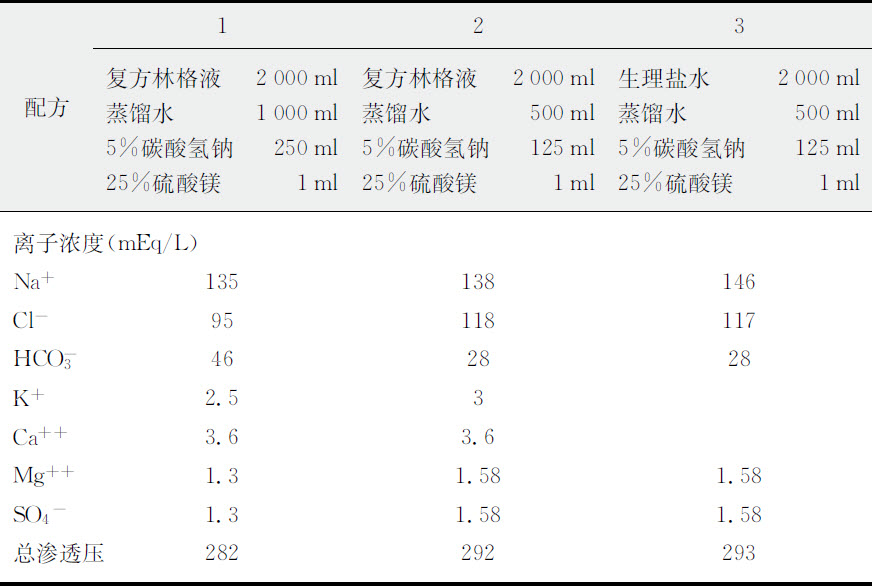
\includegraphics{./images/Image00094.jpg}
\end{table}



对于低蛋白血症患者,可考虑补充一定量的白蛋白或新鲜血浆。另外有人提出,每2~4L滤液中,有2.7~3.0g的氨基酸丢失,因此在治疗结束前也可以适当补充氨基酸。

\subsubsection{乳酸盐与碳酸盐置换液有何不同?}

尽管乳酸盐置换液对急性肾衰竭合并多器官功能障碍综合征患者代谢和血流动力学参数具有不利影响,包括增加蛋白分解,减少ATP产生等。但除了部分重症肝衰竭或乳酸酸中毒患者,仍可采用乳酸盐置换液。

碳酸氢盐置换液是最符合生理的置换液,急性肾衰竭合并多器官功能障碍综合征及高容量持续静-静脉血液滤过时应采用碳酸氢盐置换液,显然不宜用乳酸盐置换液,但在临床应用中应注意几个问题:商品化碳酸氢盐置换液由两部分组成,其中碳酸氢钠溶液应贮存于特制的包装袋内以免挥发,临用前将两者混和,切不可单独输入其中一部分;\ce{HCO3-}
水平应高于间歇血液透析使用的32~34mol/L,推荐量为35mmol/L,以便更好地控制酸中毒;置换液中不含有磷酸盐,连续肾脏替代治疗时可清除磷酸盐,应注意及时补充。前瞻性随机对照研究发现,分别采用碳酸氢盐置换液及乳酸置换液进行持续静-静脉血液滤过,碳酸氢盐置换液能更好地纠正酸中毒并降低心血管事件的发生。

\subsubsection{连续肾脏替代治疗如何实施前稀释和后稀释?}

根据置换液的补充途径分为前或后稀释。在滤器前的动脉管道中输入,即前稀释法,其优点是可以降低血液黏滞度,从而使滤器内不易发生凝血,肝素的使用量相对减少,可控制静脉端的胶体渗透压不致过高,但其要求置换液的使用量较大,滤过液中的溶质浓度低于血浆,当每天超滤量低于10L时,前稀释影响超滤效果。另外一种方法是在滤器后的静脉管道中输入置换液,即后稀释法,此种方法可节省置换液的用量,滤过液中溶质的浓度几乎与血浆相同,但在血细胞比容>45%时不宜采用,否则容易发生凝血。临床上一般应根据患者的具体情况选择补液途径和置换液的输入量。

置换液的输注量由液体出入平衡决定,每小时输注量确定后,由输液泵均匀输注。

\subsubsection{连续肾脏替代治疗不同滤过膜有何特点?}

聚丙烯腈膜(Polyacrylo
nitrile,PAN)、聚酰胺膜(Plyamide,PA)、聚砜膜(Polysulofone,PS)和聚甲基丙烯酸酯膜(Polymethyl
methylacrylated,PMMA)的生物相容性较好,体外研究已证明它们引起的炎症反应(对补体及外周白细胞激活)较小,对炎性介质的吸附性能更好。

有关透析膜对急性肾衰竭预后影响的研究不多,而且研究的样本量均较小,无法得到较肯定的结论。荟萃分析显示,应用合成膜及铜仿膜患者存活率分别为62%、55%(\emph{P}
=0.03),肾功能恢复率分别为53%、50%(\emph{P}
=0.18)。合成膜较传统的赛珞璐膜(铜仿膜)更有利于改善急性肾衰竭患者的预后。所以专家建议合成膜更适用于急性肾衰竭的肾替代治疗。

选择滤过膜时还应考虑膜的吸附功能。目前认为急性肾衰竭合并多器官功能障碍综合征时清除败血症的炎症介质可能有治疗作用。高通量膜对很多炎症介质的筛选系数均很低,如肿瘤坏死因子(TNF-α)三聚体为0.01~0.09,可溶性TNF受体为0,白介素-8为0.05~0.09,血小板活化因子为0~0.30,通过对流难于有效清除,需采用吸附。AN69膜全层中的聚合链均与血液接触,加上甲代烯丙基磺酸盐的强负荷,具有很强的吸附性。AN69膜截留分子质量为35~40千道尔顿。因此,在连续肾脏替代治疗时使用AN69膜可同时发挥弥散、对流与吸附作用。在利用吸附机制时必须同时应用超滤,并需12~24小时更换滤器,过长时间地使用可能降低膜的清除效率及其生物吸附性能。

\subsubsection{连续肾脏替代治疗时如何选择抗凝剂?}

为了保证血液滤过过程中有效的溶质清除率及滤器足够的使用寿命,抗凝是必需的。连续肾脏替代治疗过程中抗凝方法的选择应当根据病人的特征、医生的经验、监测的难易、药物的配制(包括置换液的配制)决定。现有的抗凝方法包括全身性抗凝、体外局部抗凝与无抗凝剂等,所用的抗凝剂有标准肝素、低分子肝素、直接的血栓素抑制剂(hirudin,argatroban)、枸橼酸。至于该将何种抗凝剂作为首选制剂用于连续肾脏替代治疗,目前无法达成共识。全身性凝血障碍的高危患者、已有出血及显著凝血功能障碍者需要行连续肾脏替代治疗,如何选择合适抗凝剂是非常重要的。对具有高危出血倾向的患者,肝素抗凝与出血事件和病死率显著相关,可以采用不用抗凝剂或局部枸橼酸抗凝。枸橼酸抗凝不仅出血发生率低,滤器使用时间延长,而且能降低肝素抗凝所致的血小板减少症。

虽然有多种抗凝剂可供选择(表\ref{tab12-3}),但临床上最常用的抗凝物质是肝素,可根据不同的病情适当选择使用。

\begin{table}[htbp]
\centering
\caption{连续肾脏替代治疗的抗凝药物选择及用法}
\label{tab12-3}
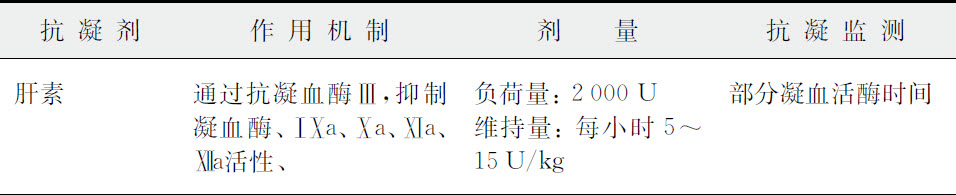
\includegraphics[width=\textwidth,height=\textheight,keepaspectratio]{./images/Image00096.jpg}
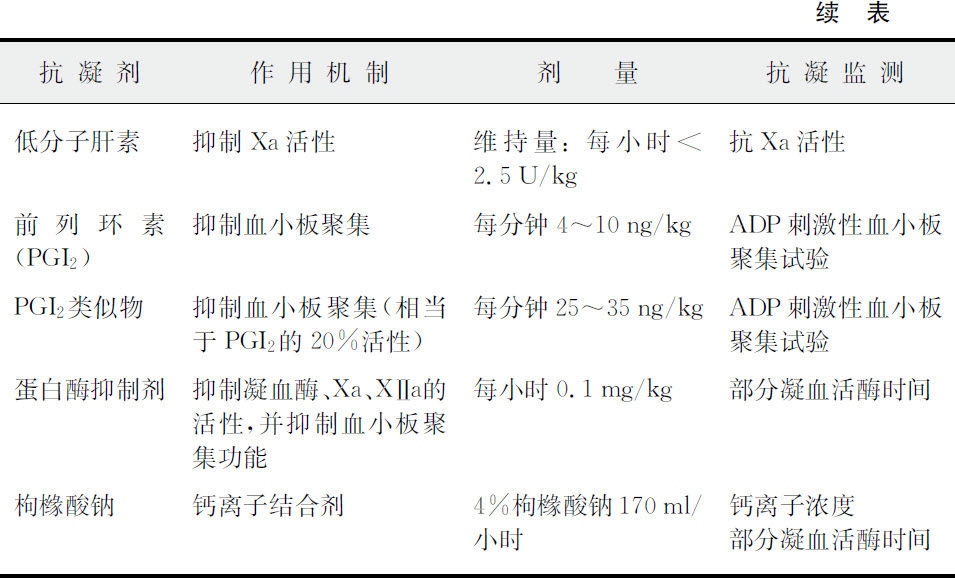
\includegraphics[width=\textwidth,height=\textheight,keepaspectratio]{./images/Image00097.jpg}
\end{table}

\subsubsection{连续肾脏替代治疗常用的抗凝方法有哪些?}

(1)全身肝素抗凝法 肝素抗凝仍是连续肾脏替代治疗中最常用的抗凝方法,常用剂量为首次剂量20U/kg,维持量为每小时5U~15U/kg或500U/小时,大部分患者可获得满意的抗凝效果。优点是使用方便,易于操作,过量时可用鱼精蛋白迅速中和;缺点是出血发生率高,药代动力学多变,血小板减少等。

(2)局部肝素化法 滤器动脉端输入肝素,静脉端输入鱼精蛋白,保持滤器中部分凝血活酶时间(APTT)在130秒左右。治疗中需分别从肝素后动脉端、鱼精蛋白后静脉端及肝素前动脉端抽血监测凝血酶原时间及部分凝血活酶时间。每100U肝素需鱼精蛋白0.6~2mg中和,鱼精蛋白需要量可应用中和试验调整,随个体和治疗时间的变化而变化。优点是对全身凝血状态影响较小;缺点是操作复杂,技术要求高,可能出现过敏反应和肝素反跳。

(3)低分子肝素法 低分子肝素是一类新型抗凝药物,抗\emph{Ⅹ}
a因子的作用强于抗Ⅱa。有较强的抗血栓作用,而抗凝血作用较弱,具有出血危险性小、生物利用度高及使用方便等优点,是一种理想的抗凝剂。低分子肝素(抗\emph{Ⅹ}
a活性)首剂静脉注射15U~20U/kg,维持剂量每小时7.5U~10U/kg静脉泵入。依据抗\emph{Ⅹ}
a因子水平调整剂量,而监测部分凝血活酶时间对调整低分子肝素剂量无帮助。低分子肝素的缺点是用鱼精蛋白不能充分中和,监测手段较复杂。

(4)无肝素抗凝法 在高危出血及出凝血机制障碍的患者可采用无肝素抗凝法行连续肾脏替代治疗。无肝素连续肾脏替代治疗最好采用生物相容性好的滤器。首先用含肝素5000U/L的生理盐水预充滤器和体外循环通路,浸泡10~15分钟,连续肾脏替代治疗前用生理盐水冲洗滤器及血路;血流量保持在200~300ml/分,每15~30分钟用100~200ml生理盐水冲洗滤器,适当增加超滤去除额外冲洗液;应用前稀释方法补充置换液。对于高危出血及出凝血机制障碍的患者使用无肝素抗凝技术不失为一种安全的选择,缺点是易出现容量超负荷及滤器堵塞。

(5)前列腺素抗凝法 前列腺素通过阻止血小板粘附和聚集功能而发挥抗凝作用,已在常规透析中成功应用。有人认为其比肝素抗凝法更安全,半衰期极短(2分钟)。但停用2小时后仍有抗血小板活性且无中和制剂,剂量调整需依靠血小板聚集试验,特别是有比较高的剂量依赖性低血压发生率,这些缺点限制了其在连续肾脏替代治疗中的应用。

(6)局部枸橼酸盐抗凝法 本法在常规透析中已显示出很多优越性,但该技术的顺利进行需以强大的弥散作用清除枸橼酸钙作为基础。推荐从动脉端输入枸橼酸钠(速度为血流量的3%~7%),从静脉端用氯化钙中和。为了避免代谢性碱中毒和高钠血症,须同时使用低钠(117mmol/L)、无碱基及无钙透析液。该技术优点是具有较高的尿素清除率和滤器有效使用时间长,缺点是代谢性碱中毒发生率高,需监测游离钙、血气等。

\subsubsection{连续肾脏替代治疗时应用肝素抗凝的具体方法和注意事项有哪些?}

(1)常规肝素抗凝法 肝素用量个体变动较大。参考用法建议为首剂量1000~3000U或20U/kg于动脉管路,以后持续注入每小时5~15U/kg。每4小时检测一次部分凝血活酶时间(APTT)。部分凝血活酶时间延长达到正常值的两倍,可获得充分的抗凝效果。

(2)存在潜在出血的抗凝 完整的血管通路,可控制的潜在出血部位(表面伤口、引流好伤口、易控制的血肿),推荐用肝素作为预防血栓栓塞并发症和作为急性肾衰竭高凝治疗量。首剂15~25U/kg,继续持续泵入每小时10U/kg,调整剂量使部分凝血活酶时间比正常值延长15秒。

(3)出血倾向明显患者的抗凝 有易出血倾向,尤其是多发创伤、外科手术后,首剂5~10U/kg,继续持续泵入每小时5~10U/kg。调整剂量使部分凝血活酶时间达到正常值便可。

凝血机能异常,血小板<10×10\textsuperscript{9}
/L,且部分凝血活酶时间延长,可用前稀释法,不必应用肝素。

肝素等抗凝剂应使用注射器泵均匀输入,输注部位应在血滤器前,以保证滤器及管路内不发生凝血。

需要监测肝素使用的并发症。最常见的是出血。据报道,持续静脉-静脉血液滤过中与肝素相关的出血发生率为5%~30%不等。若血小板计数下降,还应警惕肝素引起的血小板减少。

\subsubsection{实施连续肾脏替代治疗时,如何进行抗凝监测?}

应包括对滤器使用寿命、抗凝效果及并发症的监测。为了滤器使用寿命尽可能长,并且达到有效的清除疗效、又不使滤过膜对血细胞有破坏作用,应早期认识到滤器功能下降,比如:连续3小时滤出液减少150~200ml/小时,除外血流动力学变化的影响因素,提示滤器或管道将要堵塞。也可以每12小时检测滤出液/血尿素氮浓度比值,若低于0.7,应考虑更换滤器及管道,否则,滤出效果将显著降低,并且副作用将更加突出。

实验监测主要有滤器后的部分凝血活酶时间(APTT)、外周血血小板记数,也有用活化的凝血时间等。比较而言,APTT因监测值精确,且与肝素用量出血并发症相关性强,故较广泛应用,但其测定需要离心、且在血浆内测定,不能很好地反映肝素对全身血小板及白细胞的副作用,并且因为商品试剂差异对肝素敏感不同,有人指出,APTT作为监测肝素的标准方法需要个体试剂标准化。活化的凝血时间较为简便,床边测定速度快,但测量值范围太宽,与肝素用量相关性低于部分凝血活酶时间,故而推荐结合监测部分凝血活酶时间和活化的凝血时间。需要指出的是,因为个体对肝素作用的差异很大,监测肝素血液浓度是没有意义的。

枸橼酸抗凝后监测指标包括滤器后和血清中的离子钙水平测定,并应依此水平调整枸橼酸用量、钙的补充,同时应当监测患者的酸碱平衡指标;低分子肝素抗凝的监测指标主要是抗Xa因子活性。

滤器凝血征象的判断:①滤液尿素值/血尿素值<0.7(正常1.0),表示滤液与血液溶质不完全平衡,提示滤器内凝血。②最大超滤<100ml/小时,表示凝血,应更换滤器。③滤器前压力过高,引起管道搏动。

\subsubsection{实施连续肾脏替代治疗时,怎样进行液体平衡的管理?}

(1)液体平衡的计算 血液滤过时,患者的液体平衡应将所有的入量和所有的出量考虑在内。一般来说,每小时入量包括同期输注的置换液量、静脉输液量等(病情较轻的患者应包括口服的液体量);每小时出量包括同期超滤液量和其他途径的液体丢失量(尿量、引流量、皮肤蒸发和呼吸等)。

每小时的液体平衡=同期入量-同期出量。结果为正值为正平衡,即入量超过出量;结果为负值则为负平衡,即入量少于出量。

血液滤过等连续肾脏替代治疗期间,一般每小时计算一次液体平衡,以免患者血容量出现异常波动。

(2)液体平衡的估计 当患者接受血液滤过等连续肾脏替代治疗时,必须明确患者的容量状态,确定液体平衡的方向和程度,即液体应正平衡还是负平衡,如采用负平衡,则需明确每小时负平衡的量。由此可见,确定患者的容量状态及治疗目的是十分必要的。

患者容量状态首先可通过患者的病史、症状、体征等判断,如有困难,则应放置中心静脉导管或Swan-Ganz肺动脉导管,以监测中心静脉压、肺动脉压、肺动脉嵌顿压、心输出量等指标,明确患者的容量状态。当患者处于低血容量状态时,血液滤过时应保持适度的正平衡。

当患者血管内容量低、而第三间隙有大量液体聚集时,为减轻第三间隙的液体积聚,并提高血管内容量,则可在补充白蛋白、血浆等胶体溶液的同时,在血压和组织灌注能够维持稳定的基础上,设定血滤期间的液体平衡为零平衡或负平衡。

(3)液体平衡的仪器管理 当使用Prisma等新型床边血滤机时,医师只需设置平衡量和超滤液量等参数,机器的自动液体平衡装置则能自动调节置换液的速率,达到临床治疗要求。操作极为简便。

如只有简易血泵和输液泵,也可以较好地控制血滤的出入量。具体做法是:首先控制置换液的输注速度,由1~2个输液泵控制(置换液泵);其次控制超滤液的滤出速度,血滤器的超滤液引流管连接1~2个输液泵(超滤液泵),通过输液泵控制超滤液的滤出速度;第三,控制静脉输液的速度,营养液等静脉输液均通过输液泵静脉输入(静脉输液泵),以控制输注速度;最后,可计算液体平衡,液体平衡=(置换液泵量+静脉输液泵量)-(超滤液泵量+其他出量)。

通过以上方法,可做到血滤期间准确、有效的液体平衡管理,使危重患者连续肾脏替代治疗更为安全。

\subsubsection{影响血液滤过超滤的因素有哪些?有何临床意义?}

影响超滤率的关键是滤过压(跨膜压),其次为血流量。在持续静脉-静脉血液滤过中影响跨膜压的因素如下。

(1)滤液侧负压 是产生超滤的主要因素之一,负压的大小取决于滤过器与滤液收集袋之间的垂直距离:负压=高度(cm)×0.74mmHg。因此,滤液收集袋的位置通常低于滤器20~40cm。若在滤液侧加一负压吸引器,则可以提高超滤率。但应注意负压不可太高,以防滤膜破裂。

(2)静水压 滤器内的静水压与血流速度有关,血流速度越高,滤器内的静水压越高,而静水压越高,超滤量越大。持续动-静脉血液滤过时,静水压主要与平均动脉压有关。

(3)胶体渗透压 血浆胶体渗透压是跨膜压的反作用力,胶体渗透压越高,跨膜压便越低。当胶体渗透压等于滤液侧负压和静水压时,超滤便停止进行。胶体渗透压受血浆蛋白浓度的影响。

(4)血液黏度 血液黏度决定于血浆蛋白浓度及血细胞比容,当血细胞比容>45%时,超滤率可降低。

此外,还有一些其他的因素,如血液通道的长度,静脉侧的阻力,滤器等均可以影响超滤的速度。一般在治疗的初期,超滤的速度为10ml/分以上,低于5ml/分则应注意患者的血压,管道有无扭曲,滤器有无破膜漏血,滤液收集袋的位置是否合适等。

\subsubsection{连续肾脏替代治疗和间歇血液透析对急性肾衰竭预后有无不同影响?}

从理论上讲,连续肾脏替代治疗血流动力学相对稳定,应用生物相容性高的膜材,有利于肾功能恢复;间歇血液透析过程中易反复发生低血压,导致肾脏灌注压下降,促进肾小管细胞坏死或阻碍原有坏死肾小管细胞修复,透析膜生物相容性差也影响肾功能恢复,因此,以连续肾脏替代治疗重症患者急性肾衰竭可能优于间歇血液透析。但Vinsonneau等
\protect\hyperlink{text00018.htmlux5cux23ch11-17}{\textsuperscript{{[}11{]}}}
进行的21个重症医学科、360例患者的多中心研究结果发现,在合并急性肾衰竭的重症患者中,随机进行连续肾脏替代治疗或间歇血液透析治疗,两组的病死率无明显差异(连续肾脏替代治疗组33%,间歇血液透析组32%)。近期的Meta分析
\protect\hyperlink{text00018.htmlux5cux23ch12-17}{\textsuperscript{{[}12{]}}}
同样提示,连续肾脏替代治疗并不能比间歇血液透析更好地改善患者的肾功能或降低病死率。因此,目前并无充分的证据表明在急性肾衰竭的患者中,连续肾脏替代治疗比间歇血液透析更能改善预后。

\subsubsection{连续肾脏替代治疗在急性肾衰竭中的应用指征是什么?}

目前,连续肾脏替代治疗复杂性急性肾衰竭患者的适应证及最佳时机,尚无统一标准,大多数学者基本出发点是当内科治疗失败,患者出现尿毒症或水电解质失衡时,才开始给予连续肾脏替代治疗,这种标准对于病情相对稳定或单纯性急性肾衰竭可能是合理的,但对于重症医学科复杂性急性肾衰竭患者是十分危险的。

一般认为重症急性肾衰竭患者应采用连续肾脏替代治疗。鉴于重症急性肾衰竭患者达到传统透析指征后开始透析预后更差,所以重症急性肾衰竭患者应当在传统透析指征出现之前就要开始连续肾脏替代治疗。重症脑外伤、脑外伤手术病人和急性肝衰竭病人发生急性肾衰竭时常伴有脑水肿,间歇血液透析治疗有致命性的危险。比如间歇血液透析易导致失衡综合征,脑水肿加重,颅内压升高,脑血流灌注压下降,甚至发生脑疝和死亡。因此,对于有脑水肿或具有脑水肿高危因素的患者,间歇血液透析是绝对禁忌证。而连续肾脏替代治疗则可以维持脑灌注压,不会引起颅内压升高,患者能够耐受连续肾脏替代治疗,因此,可以应用连续肾脏替代治疗来救治这类患者。

决定开始连续肾脏替代治疗的标准是依据患者临床病情(如其他器官的损害情况),而不是依据生理指标是否达到尿毒症水平。决定是否开始连续肾脏替代治疗时,水负荷比氮质血症更重要,否则,如果患者发展到多器官功能障碍综合征阶段,则治疗已晚,代价大,病死率高。早期或预防性连续肾脏替代治疗能更好地控制水电解质酸碱平衡,促进肾功能恢复,改善复杂性急性肾衰竭的预后。

目前认为,连续肾脏替代治疗具体指征分为肾脏替代治疗及器官支持治疗两部分。

(1)肾脏替代治疗指征 ①急诊治疗指征------高钾血症,酸中毒,肺水肿;②尿毒症并发症;③控制溶质水平;④清除液体;⑤调节酸碱和电解质平衡

(2)多器官支持治疗指征 ①营养支持;②急性心衰时清除液体;③心肺旁路时清除液体与炎症介质;④脓毒症时调节细胞因子平衡,重建机体免疫内稳状态;⑤ARDS时纠正呼吸性酸中毒,清除水分与炎症介质;⑥多器官功能障碍综合征时的液体平衡;⑦挤压综合征时清除内源性毒性物质;⑧肿瘤溶解综合征时清除尿酸和磷。

\subsubsection{肾脏替代治疗的充分性如何判断?}

肾脏替代治疗的充分性反映了替代治疗对代谢产物的清除效率和血浆中代谢产物降低的程度。美国透析研究协作组(NCDS)提出将尿素氮作为衡量透析充分与否的小分子溶质清除指标。近年来,将β\textsubscript{2}
微球蛋白的清除作为大分子溶质清除是否充分的指标。

首先计算透析前后的血浆尿素氮比值(R),R=透析后血尿素氮/透析前血尿素氮,反映尿素清除效果;其次计算尿素下降比值(urea
reduction
ratio,URR),URR=1-R。URR越高,说明血尿素氮清除越多,透析效果越好。最后,计算尿素清除指数(KT/V),其中K为尿素氮清除率、T为透析时间、V为尿素的分布容积。可根据经验公式计算KT/V=1.18×[-In(R)]。

当KT/V<0.8(R>0.5)时,患者并发症多,而且病死率高。KT/V=1.0(R<0.42)为一般可接受的最低KT/V和R标准。目前认为,KT/V=1.2~1.3,才表明透析充分。可见,监测连续肾脏替代治疗的充分性很有必要。但目前对于连续肾脏替代治疗的充分性尚缺乏可靠的评价手段。

\subsubsection{如何选择肾替代手段治疗严重感染及其导致的急性肾衰竭?}

严重感染致急性肾衰竭者有58%~70%需肾替代治疗,伴急性肾衰竭者病死率为53%~73%,采用何种方式降低病死率与恢复肾功能是当前研究的重点。

病原菌侵入机体后,大量的促炎因子和抗炎因子释放,进而导致全身炎症反应失衡在感染的发生发展过程中发挥着重要作用。因此有效地清除炎症因子和毒素,进而调节全身炎症状态,可能能够改善重症患者的病情。常见的炎症因子如白介素-1β、白介素-6、白介素-8、肿瘤坏死因子-α等多为中大分子物质,主要通过吸附及对流的原理进行清除;而脂多糖、肿瘤坏死因子-α多聚体等分子量更高,仅能通过吸附进行清除,因此可以采用血液滤过、血浆吸附、血液灌流等模式治疗重症感染患者。

血液滤过通过对流的方式清除溶质,对中分子量的炎症因子清除效果较好。Ronco等
\protect\hyperlink{text00018.htmlux5cux23ch13-17}{\textsuperscript{{[}13{]}}}
研究发现,在急性肾衰竭的患者中,持续血液滤过治疗剂量从每小时25ml/kg增加至35ml/kg时,患者存活率从41%明显上升至57%,而治疗剂量再增加至每小时45ml/kg时,患者存活率并未出现明显改善(58%);而对感染患者进行亚组分析显示,持续血液滤过治疗剂量从每小时25ml/kg增加至每小时35ml/kg时,患者存活率分别为25%、18%,而治疗剂量再增加至每小时45ml/kg时,患者存活率明显升高至47%。可见在重症感染的治疗中,连续肾脏替代治疗的治疗剂量与常规肾脏疾病的治疗剂量有所区别,高流量血液滤过更适用于重症感染的治疗。但进一步的研究并未发现更高的连续肾脏替代治疗的治疗剂量能进一步改善重症感染合并急性肾衰竭患者的预后。

\subsubsection{如何评价连续肾脏替代治疗在严重感染清除炎症介质的地位?}

应用连续肾脏替代治疗清除循环中的炎症介质,近30年来进行了大量的实验研究与临床探索,陆续提出了一些假说,深化了我们对严重感染发病机理的认识,发展了一些新的连续肾脏替代治疗技术,并进行了有益的尝试。

由于严重感染病人基础病、自身防御机制受损和免疫失调程度不同,治疗时间各异,目前还没有快速测定细胞因子的方法,无法判断炎症反应的时期,难以适时地应用特异性清除方法,无法进行前瞻性对照研究,因此很难判断临床疗效。特别是以后的研究认为,促炎症介质与抗炎症介质之间形成复杂的网络,细胞因子生成失控,连续肾脏替代治疗的目的是将失控的过高的各细胞因子控制在适当水平,即Ronco等提出的高峰浓度假说。

滤过膜的孔径不是均匀一致的,截留分子量是指平均膜孔直径滤出的溶质分子量,一些分子量大于截留分子量的溶质仍能被少数大于平均膜孔直径的膜孔滤出,提高血液滤过的容量和增加更换滤器的频率可增加大分子溶质的清除。大量的动物及临床研究结果均提示,在严重感染模型或患者中,连续肾脏替代治疗能够明显降低白介素-1β、白介素-6、白介素-8、肿瘤坏死因子-α等炎症因子水平,但患者的预后并未得到有效的改善。可能与炎症反应时大量促炎和抑炎因子形成复杂的网络关系,单纯清除某一种或几种炎症因子无法彻底逆转严重感染的进程有关。因此,常规流量的连续肾脏替代治疗无效时,可试用高流量血液滤过进一步增加治疗剂量治疗严重感染和感染性休克。

\subsubsection{在什么情况下,可考虑终止连续肾脏替代治疗?}

与所有治疗类似,当临床重症患者开始肾脏替代治疗时,需要考虑在何时终止该治疗。一方面肾脏替代治疗存在有益物质丢失、凝血功能异常等并发症;另一方面,患者或医疗保险经济负担增加、患者生活质量降低,因此在患者病情好转、条件许可时也应尽早撤离肾脏替代治疗。Uchino等
\protect\hyperlink{text00018.htmlux5cux23ch14-17}{\textsuperscript{{[}14{]}}}
对23个国家的54家重症医学科的1006例连续肾脏替代治疗的急性肾损伤患者进行前瞻性观察性研究,发现患者尿量增加、代谢紊乱纠正、容量负荷过多改善、尿素氮或血肌酐水平下降及血流动力学稳定等均是临床考虑停止连续肾脏替代治疗的指征。统计学分析发现,尿量明显增加、血肌酐下降是预测肾脏替代治疗能够成功撤离的指征。在无利尿剂干预情况下24小时尿量>400ml或在利尿剂干预下24小时尿量>2300ml的患者中,约80%能够成功撤离连续肾脏替代治疗。此外,研究也发现,成功撤离肾脏替代治疗的患者比不能成功撤离肾脏替代治疗患者的病死率明显下降,重症医学科时间及住院时间显著缩短。因此,选择更好的时机撤离肾脏替代治疗尤为重要。但目前对肾脏替代治疗撤离时机的资料仍十分缺乏,临床更多的是在需要行肾脏替代治疗的原发疾病得到控制,肾脏功能逐步恢复,患者病情明显改善时按照经验选择肾脏替代治疗撤离时机,但标准并不统一。尿量、血肌酐水平可以作为急性肾损伤患者肾脏替代治疗撤离的敏感参考指标。而其他疾病的肾脏替代治疗的撤离时机仍需要大规模的随机对照研究证实。

\subsubsection{连续肾脏替代治疗有哪些新技术?有何临床意义?}

经典的连续肾脏替代治疗技术在重症患者的代谢和体液平衡控制中发挥了重要作用,也能清除一些细胞因子,但血浆细胞因子的浓度并未显著下降,可能与治疗剂量的选择、滤器的筛选系数以及滤过率降低、膜的吸附作用饱和、溶质的对流转运较为有限有关。近来有学者报道,将不同血液净化方式联合应用,取得一定的临床疗效。

血液灌流+血液透析(hemoperfusion
hemodialysis,HPHD)既能够通过血液灌流吸附各种特异和非特异性毒素,又能解决水电解质、酸碱平衡的问题。但其缺陷为吸附能力在4小时达到饱和,清除能力下降。

持续性血浆滤过吸附(continuous plasma filtrationad
sorption,CPFA)将血液引出体外后,先用血浆分离器分离血浆,血浆经树脂和活性炭吸附后再与血细胞混合,进行血液滤过。持续性血浆滤过吸附综合了血浆吸附和血液滤过的优势,能够有效清除炎症介质,成为重症感染治疗的有效措施之一。

高容量血液滤过(high-volume
hemofiltration,HVHF)也是近几年出现的新技术。高容量血液滤过显著加大了置换液输入量及单位时间血流量,使大、中分子炎症介质的对流和吸附清除均增加,下调炎症反应,对于阻止甚至逆转多器官功能障碍综合征进程,以及改善相应的临床症状均有明显效果。

多黏菌素B血液灌流(direct hemoperfusion with polymyxin B-immobilized
fiber
column,DHP-PMX)通过将多黏菌素B固定到聚苯乙烯纤维中,行血液灌流治疗重症感染患者,能够有效地清除患者体内的内毒素水平,调节全身炎症反应状态,进而改善患者的血流动力学、氧合,降低患者病死率。多黏菌素B血液灌流既发挥了多黏菌素B特异性结合内毒素的特性,又避免了药物的不良反应,Cruz等
\protect\hyperlink{text00018.htmlux5cux23ch15-17}{\textsuperscript{{[}15{]}}}
在腹腔重症感染的患者中应用多黏菌素B血液灌流治疗后,患者28天病死率为32%,而对照组为53%(\emph{P}
<0.05),并且治疗组患者的血流动力学改善更明显,对血管活性药物依赖程度降低,序贯器官衰竭评分降低。因此,在重症感染,尤其是革兰阴性杆菌感染的治疗中,多黏菌素B血液灌流可能发挥重要作用。

由于不同血液净化方式均有其独特的清除特点,故不同方式的联合应用可能是血液净化治疗发展的必然趋势。

\subsubsection{何谓血浆滤过吸附?有何临床意义?}

不少炎症介质难以通过连续肾脏替代治疗的滤过膜,即使采用高容量血液滤过也不可能清除肿瘤坏死因子和白细胞介素-10等大分子的介质。要清除这些介质,只有用吸附手段。现有的吸附剂如树脂或活性炭,用生物相容性好的物质包被,提高了生物相容性,但对吸附性能影响较大。用多聚体包被活性炭后,被吸附溶质的最大分子量从21500道尔顿降至3500道尔顿。

联合血浆滤过吸附(CPFA)是将血液引出体外后,先用血浆分离器分离血浆,血浆经不包被的树脂和活性炭吸附,吸附后的血浆再与血细胞混合进行血液透析滤过。

一次通过吸附剂后血液中肿瘤坏死因子与白介素-10被100%吸附。联合血浆滤过吸附治疗后病人单核细胞在无刺激和脂多糖刺激下生成肿瘤坏死因子α量随治疗时间延长而增加,治疗后最高(\emph{P}
=0.009),表明免疫麻痹现象改善。一项前瞻性临床研究
\protect\hyperlink{text00018.htmlux5cux23ch16-17}{\textsuperscript{{[}16{]}}}
表明,与单独持续静-静脉血液滤过相比,联合血浆滤过吸附治疗后严重感染性休克患者的平均动脉压显著升高(\emph{P}
=0.001),去甲肾上腺素用量明显减少(\emph{P} =0.003)。Formica等
\protect\hyperlink{text00018.htmlux5cux23ch17-17}{\textsuperscript{{[}17{]}}}
亦发现联合血浆滤过吸附不仅能够降低重症感染患者血肿瘤坏死因子及白介素-10水平,而且改善患者血流动力学状态,提高患者生存率。由此可见,联合血浆滤过吸附可能通过有效清除炎症介质而成为治疗感染性休克的有效手段。

\subsubsection{连续肾脏替代治疗时药物代谢及药效的影响因素有哪些?}

连续肾脏替代治疗发挥有效治疗作用的同时,对药物也起到清除作用。因此,在连续肾脏替代治疗的同时也要保证药物治疗的有效性与安全性。连续肾脏替代治疗时影响病人药物代谢及药效的因素有药物因素、病人因素、滤器及血液净化的方式和相关参数。

(1)药物因素 ①分子量:在连续肾脏替代治疗过程中由于采用合成膜滤器,且采用对流转运的原理,其药物清除率接近于血浆药物的非蛋白结合率。通常分子量<500道尔顿的小分子在传统血透可有效清除,分子量1000~5000道尔顿者连续肾脏替代治疗可有效清除。②尿液中药物原型清除比率:主要以原型形式经肾脏排泄的药物,在开始连续肾脏替代治疗后总体清除率可能较连续肾脏替代治疗前有较为明显的增加,而主要以非肾脏途径排泄的药物其总体清除率则在连续肾脏替代治疗前后可能无明显变化。③药物分布容积:该容积过大则可能在特定组织或器官中蓄积。连续肾脏替代治疗由于治疗时间的延长,可为组织与血管间药物转移提供时间,因而可显著影响该类药物的总体清除效率。④血浆蛋白结合率:血浆蛋白结合率的高低,影响药物在体内的分布和转运速度、作用强度及清除速率。血浆蛋白结合率高的药物,由于药物-蛋白结合的复合物分子量多>50000道尔顿,因此无论传统血透还是连续肾脏替代治疗,其清除效率均较差。

(2)病人因素 ①病人残余肾功能:较为准确地评价连续肾脏替代治疗对病人总体清除率的影响;②病人容量状况;③其他脏器功能状态,尤其肝功能状态对于药物的清除、蛋白结合、分布容积均有影响。

(3)滤器对药物清除的影响 滤器影响连续肾脏替代治疗药物清除的主要因素为超滤率、滤器的筛选系数。

(4)血液净化的方式及相关参数 血液净化方式(如持续静-静脉血液滤过、持续静-静脉血液透析、持续静-静脉血液滤过透析等)不同,药物清除率不同。取决于透析液或血滤置换液的流量、超滤率及血流量的大小。持续静-静脉血液滤过、持续静-静脉血液滤过透析药物清除率优于持续静-静脉血液透析。

以上多种因素共同影响连续肾脏替代治疗时药物代谢及药效,因此,连续肾脏替代治疗时药物代谢是一个非常复杂的过程。

\subsection{血液透析基本原理和实施}

\subsubsection{血液透析基本原理是什么?与血液滤过有何不同?}

血液透析(hemodialysis)疗法是根据膜平衡的原理,将患者血液通过半透膜与含一定成分的透析液相接触,两侧可透过半透膜的分子(如水,电解质和中小分子物质)做跨膜移动,达到动态平衡,从而使血液中的代谢产物,如尿素、肌酐、胍类等中分子物质和过多的电解质,通过半透膜弥散到透析液中,而透析液中的物质如\ce{HCO3-}
和醋酸盐等也可以弥散到血液中,从而清除体内有害物质,补充体内所需物质的治疗过程。

血液透析中的溶质运转方式有两种:①弥散,即溶质从高浓度处向低浓度处运动。溶质运动的动力来自其本身无规则的热运动,即布朗运动。影响弥散运动的因素包括溶液浓度梯度、溶质分子量和半透膜的阻力。②超滤,即液体在压力梯度作用下通过半透膜的运动。当膜的一侧液面压力大于另一侧时,在膜的两侧产生流动压差(跨膜压),使小分子从加压一侧向不加压的一侧做跨膜移动,小分子溶质以原溶液相同浓度随水分子一起通过半透膜而被清除,大分子溶质保持不变。超滤动力来自静水压及渗透压。

血液滤过主要是通过对流原理清除溶质,清除中、小分子能力相等;血液透析主要是通过弥散原理清除溶质,清除率与分子量成反比,对小分子的清除优于中分子。血液滤过对中分子的清除优于血液透析。

\subsubsection{急性肾衰竭实施血液透析的指征和禁忌证有哪些?}

(1)急性肾衰竭实施血液透析的指征 具有以下临床症状:①无尿2天或少尿3天;②每天体重增加2.0kg以上;③浮肿、肺水肿、胸水;④恶心、呕吐;⑤出血倾向;⑥神经、精神症状。或实验室检查达到以下指标:①血清肌酐>8mg/dl;②血清尿素氮>80mg/dl;③血清钾>6.0mmol/L;④血清\ce{HCO3-}
<15mmol/L;⑤血清尿素氮每天上升>30mg/dl,血清钾每天上升>1.0mmol/L。

(2)血液透析的相对禁忌证 ①休克或低血压;②严重出血倾向;③心功能不全或严重心律失常不能耐受体外循环;④恶性肿瘤晚期;⑤脑血管意外;⑥未控制的严重糖尿病;⑦精神失常及不合作患者。

\subsubsection{血液透析治疗中暂时性和永久性血管通路有何不同?}

暂时性血管通路是指在短时间内能够建立起来并能立即使用的血管通路,一般能维持数小时乃至数月以满足患者在短期内实施血液净化的治疗。适用于:急性肾衰竭达到透析指征者;进行血浆置换,血液灌流,免疫吸附,持续动静脉血滤等治疗;腹膜透析患者因透析管阻塞或隧道感染,需要拔管或植入新管期间;慢性肾衰竭患者在内瘘成熟前有紧急透析指征者或者血透患者因内瘘闭塞需要重新做瘘者。

常用建立血管通路的方法有:①直接动、静脉穿刺法(即直接穿刺外周动脉和静脉,在有困难或紧急情况时也可以经皮做深动、静脉穿刺插管。②中心静脉经皮穿刺插管,利用双腔或三腔静脉导管经皮做中心静脉穿刺插管也可满足双针透析治疗的需要,在抗凝治疗的条件下可以较长时间的保留,是目前建立暂时性血管通路的主要和首选方法。其选择途径一般是经锁骨下静脉,经颈内静脉,经股静脉实施经皮插管。临床上我们最常选用的是经皮颈内静脉插管。③动---静脉外瘘,又称为Quiton-scribner分流,上世纪60年代初期曾是透析患者的主要血管通路,近年由于中心静脉经皮插管的广泛应用,且保留时间较长,加之动静脉外瘘本身又有一定的缺点(如患者行动不便,容易感染等),已有被取代的趋势,在某些中心静脉插管有困难的医院还在继续使用。

永久性血管通路是指在血液透析中能够使用数月以至数年的血管通路,适用于维持性血液透析患者,主要包括直接动---静脉内瘘和移植血管的动---静脉内瘘,少部分为中心静脉插管长期留置和不用穿刺针的“T”形管式血管通路。

\subsubsection{血液透析治疗中永久性血管通路应注意哪些并发症?}

永久性血管通路是长期血透患者的生命线,保护好血管通路,延长使用是一个非常重要的问题。为此我们必须了解有关永久性血管通路的一些并发症。

(1)直接动---静脉内瘘

血栓形成:早期动、静脉的血栓形成是在手术后24小时内,主要原因是吻合口血管袢成角,吻合中损伤血管内膜导致吻合口水肿或吻合口过小,动、静脉外膜剥离不干净,动、静脉痉挛,患者血液高凝状态及低血压等。处理方法是早期发现,立即再次手术,正确的手术操作,术后全身抗凝治疗,肢体保温,维持正常血压等。后期血栓形成常见于过早使用尚未成熟的动---静脉内瘘,穿刺和压迫止血不当,使用促凝药物(如促红细胞生成素、环孢霉素A等),及患者发生血压下降的情况。防治办法是严格掌握内瘘的首次使用时间(一般在3~4周),避免在同一部位反复穿刺,及时减少促红细胞生成素的用量,防止出现低血压状态等。

出血:常发生于术后24小时内,多由于抗凝药物过量,吻合针距过大缝合线脱结及患者血压增高等所致。所以应适当注意抗凝药物的使用剂量,必要时应再次手术缝合,丝线打结应连续在7个以上。

假性血管瘤:主要是由于静脉血管局部扩张引起,常常提示内瘘血管不全性狭窄或局部血管壁损伤。原则上不需要处理,血管造影有助于明确血管病变的位置及大小,如有感染或破裂,应立即手术。

血流量不足:常见于静脉发育不良,曾经接受反复输液或静脉化疗以及静脉分支多的患者。处理包括鼓励患者加强术后的肢体活动,若无效则可再次手术用移植血管代替不良的血管。

感染:除手术因未严格无菌操作而发生切口感染外,内瘘穿刺部位很少发生感染,如果内瘘血管出现感染或全身性感染,应及时使用敏感的抗生素,必要时切除感染的病灶,关闭内瘘。

动---静脉分流量过大导致的心脏负荷过重:常见于心功能不全的老年患者,如果吻合口≤4mm,对心脏的影响较小,所以病情严重的患者需再次手术缩小吻合口。

(2)移植血管的动---静脉内瘘 栓塞和感染是移植血管的主要并发症,移植血管的栓塞发生率远远高于直接动---静脉内瘘;自体和异体血管的栓塞发生率远高于人工血管。另外,与移植血管的材料的生物相容性、术前处理、血管吻合技术等有关。移植血管感染的发生率也较直接动---静脉内瘘高,治疗较为困难,除需要使用大量的抗生素外,有相当一部分的患者还需要切除移植的血管。移植血管的感染主要与穿刺有关,故穿刺时应严格无菌操作。

\subsubsection{什么是血液透析首次使用综合征?如何处理和预防?}

首次使用综合征是使用新透析器产生的一组症候群,有过敏型(A型)和非特异型(B型)(表\ref{tab12-4})。

\begin{table}[htbp]
\centering
\caption{血液透析首次使用综合征的类型}
\label{tab12-4}
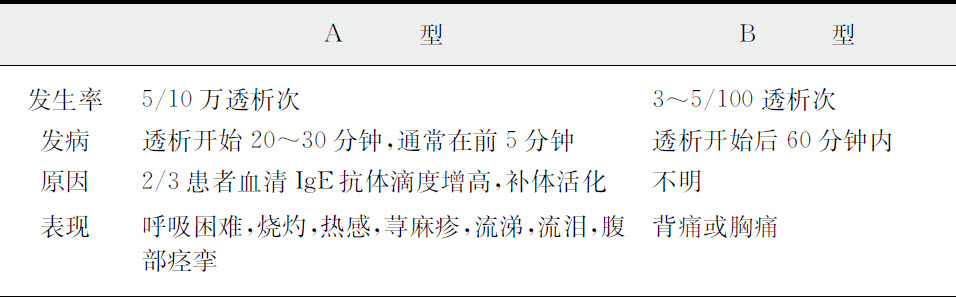
\includegraphics[width=\textwidth,height=\textheight,keepaspectratio]{./images/Image00100.jpg}
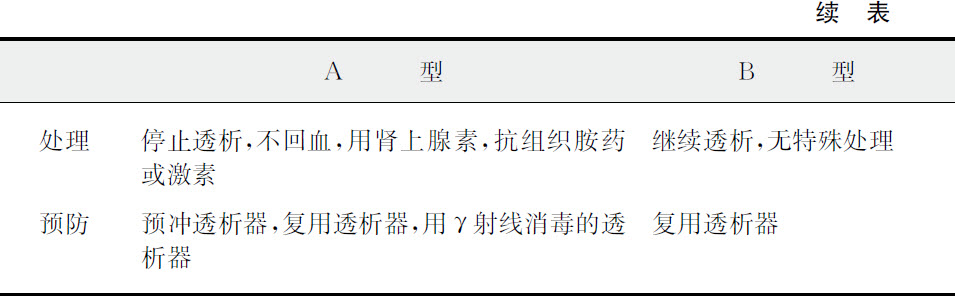
\includegraphics[width=\textwidth,height=\textheight,keepaspectratio]{./images/Image00101.jpg}
\end{table}

(1)A型反应 在透析开始几分钟内即可以发生,轻者仅表现为瘙痒、荨麻疹、咳嗽、流泪、腹痛或腹泻等。重者可出现呼吸困难、心跳骤停,甚至死亡。发生原因尚不清,可能与过敏有关。处理:对严重反应者应立即停止透析,丢弃透析器和管道内的血液。必要时应用抗组胺药、激素或肾上腺素进行治疗及抢救。

(2)B型反应 在透析开始几分钟到1小时发生,发生原因不清,主要表现为胸背痛,应注意与心绞痛鉴别。处理:主要包括吸氧及对症处置,一般不必停止透析。

透析前应用生理盐水彻底冲洗透析器可以减少此类情况发生。

\subsubsection{何谓血液透析的失衡综合征?怎样处理和预防?}

失衡综合征是指在透析中、后期或结束后不久发生的与透析有关的以神经系统症状为主的症候群。临床表现为:恶心、呕吐、不安、头痛、惊厥、意识障碍及昏迷。病因较多,主要是由于透析时血中尿素氮比脑脊液中下降的快,血脑之间产生渗透压差,使水进入脑细胞,引起脑水肿。也有人认为透析后酸中毒纠正,血红蛋白与氧的亲和力增加,导致脑缺氧也是原因之一。

预防和处理措施包括:①最好在血浆尿素氮不超过23.6mmol/L即开始透析;②首次透析采用低效透析器,时间不超过3小时,逐渐过渡;③适当提高透析液中钠浓度,静点甘露醇及50%葡萄糖是预防失衡综合征的有效方法;④已经发生失衡综合征时,轻者要缩短透析时间,重者立即停止透析,给予对症处置。对轻症患者给予静脉滴注高张溶液、镇静剂,重者应终止透析,静脉滴注甘露醇,静脉注射地西泮(安定);对昏迷者要注意呼吸道通畅。

\subsection{腹膜透析的应用}

\subsubsection{何谓腹膜透析?其基本原理是什么?}

腹膜透析(peritonealdialysis,PD,以下简称腹透)自1923年由Ganter首先用于临床以来,由于其操作简单、实用有效、价格低廉、不必全身肝素化、不需特殊设备、不需专门训练人员和安全等许多优点,已成为治疗急性或慢性肾衰竭和某些药物中毒的有效措施。腹膜透析方法随透析液交换周期的不同,分为连续循环腹透,间歇性腹透和不卧床持续性腹膜透析。临床上治疗慢性肾不全以持续性腹膜透析使用最为广泛。

腹膜是具有透析功能的生物半透膜,不仅有良好的渗透和扩散作用,还有吸收和分泌功能。成人的腹膜面积为2.0~2.2m\textsuperscript{2}
,较两侧肾脏的肾小球滤过总面积(约1.5m\textsuperscript{2}
)和一般的血液透析膜面积(0.8~1.0m\textsuperscript{2}
)为大。根据多南凡平衡原理,在半透膜两侧的溶质浓度不等时,则高浓度一侧的溶质,如其分子量较小,可通过半透膜向低浓度的一侧弥散,而水分子则向渗透压高的一侧渗透,最后达到半透膜两侧的平衡。大分子物质如大分子蛋白、血细胞等则不能通过。根据这种原理,将透析液灌入腹膜腔后,血浆中的小分子物质,如浓度高于透析液者,就会弥散入透析液内;而透析液中浓度高的物质,则可从透析液内进入组织液和血浆内;若透析液的渗透压高于血浆,则血浆中过多的水分便渗透至透析液内。因而做腹透时,通过向腹腔内反复灌入和放出透析液,就可使潴留体内的代谢产物得到清除,水和电解质得到平衡而达到治疗的目的。腹透过程中,溶质通过弥散和超滤进行运转:①弥散是溶质从高浓度处向低浓度处的运动,是腹膜清除废物的主要机制。腹透是弥散作用在腹膜表面毛细血管内血流与腹腔内腹透液之间进行。腹透液与血液之间的浓度梯度,溶质分子量及腹膜阻力影响弥散的效率。②超滤是液体在压力梯度作用下通过半透膜的运动。超滤是水分和可渗透性溶质一起通过腹膜。超滤作用由透析液与血液之间渗透压梯度决定,是透析清除水分的重要机理。

\subsubsection{慢性肾衰竭时,与血液透析相比哪些患者更适合应用腹膜透析?}

腹膜透析指征与血液透析相同,但与血液透析相比,以下患者更适合于腹膜透析:①>65岁的老年人;②原有心血管疾病或心血管系统不稳定的患者;③糖尿病患者;④有明显出血倾向患者;⑤反复血管造瘘失败患者;⑥儿童。

\subsubsection{腹膜透析应用禁忌证有哪些?}

腹膜透析在几乎所有的临床条件下都能够应用,但有时选择血液透析更为适宜。

(1)绝对禁忌证 ①腹腔感染或肿瘤等所致腹腔广泛粘连或纤维化;②腹壁广泛感染、严重烧伤或皮肤病。

(2)相对禁忌证 ①腹部手术后3天内,腹腔留置引流管;②腹腔局限性炎性病灶;③腹腔内容严重减小,如高度肠梗阻、晚期妊娠、腹腔巨大肿瘤等;④严重呼吸功能不全;⑤精神病患者或不合作者;⑥长期蛋白质及热量摄入不足者;⑦疝气、腰椎间盘突出。

\subsubsection{腹膜透析充分性的标准有哪些?}

目前认为达到透析充分性的标准除了达到足够的尿素氮、肌酐清除率外,还应达到以下各项指标:①除小分子溶质的清除外,还应达到较大分子的清除;②达到足够的超滤,维持水、电解质平衡;③纠正代谢性酸中毒;④控制钙、磷代谢的平衡及维持甲状旁腺素正常水平;⑤理想的营养标准及抗感染能力;⑥理想的血压、血脂控制及控制心血管病的发生;⑦改善贫血达理想水平。

\subsubsection{解决腹膜透析患者低蛋白血症的主要措施有哪些?}

解决低蛋白血症的主要措施是:①充分透析。研究表明,蛋白分解代谢率与尿素清除指数呈高度相关性。即增加透析剂量可使蛋白质摄取率增加,无论是血液透析或腹膜透析,都必须充分透析。②加强肠外营养,尤其是老年人因消化机能减退,活动量小,代谢下降,给予肠外营养应该是有效的手段。③补充足够热量,减少蛋白的分解代谢。④增加运动量,改善消化功能。⑤鼓励进食。

\subsubsection{腹膜透析治疗急性肾衰竭有何利弊?}

腹膜透析(简称腹透)作为一种肾替代治疗方法用于急性肾衰竭的治疗,有其独特的优点:首先,腹透设备及操作简单,安全且易于实施。与连续肾脏替代治疗相比,腹透不需要特殊的设备及血管通路。如果临床上预计肾衰竭病程短,可不需要置入带克夫的Tenckhoff导管。这样可以在床边通过穿刺法置入无克夫的临时腹透管,半小时后就可进行透析;如果估计其肾功能恢复所需的时间较长,需置入带克夫的Tenckhoff导管,其腹透交换操作可以通过机器进行,也可以通过人工进行。腹透不需要抗凝,可以避免与血管通路相关的一些问题。对于有出血倾向、手术后急性肾衰竭、外伤及颅内出血等对抗凝有禁忌的患者尤其适用。由于其连续性,可以在较长的时间内清除水分,单位时间内清除的液体量少,保证清除效果的同时有较好的血流动力学稳定性,较少发生低血压,从而减少低血压对肾脏的进一步损害,适合于治疗血液动力学不稳定或无法建立血管通路的病人。由于腹透能够持续地纠正酸中毒和电解质紊乱,逐步去除氮质潴留,因此较少引起失衡综合征。

但是腹透也存在一些技术上的不足。腹腔内有病变或近期有腹部大手术史的急性肾衰竭患者,腹透就不合适;腹腔压力增高后,横膈上抬,影响肺的通气量,对于有急性肺损伤或ARDS的患者会干扰肺的呼吸交换;腹透时,蛋白质从腹透液中丢失则会进一步加重危重患者的营养不良。

另一方面,腹透虽然操作简单,但技术上的要求并不低。不熟悉腹透的医务人员就难以取得治疗的成功。腹透是依靠患者自身的腹膜进行透析,如果腹膜受损,就无法进行。腹透如果操作不当,容易发生腹膜炎、导管相关并发症(如漂管、堵管、渗漏等),进而严重影响透析质量,甚至导致透析失败。不熟悉这项技术时采用腹透,其过程中出现并发症就会相对较多。

此外,腹透具有缓慢、持续透析的特点,对于威胁生命的高钾血症或严重的心功能衰竭等需要立即清除血钾和水分时,腹透也不易快速奏效;对于一些高分解代谢,需要清除较多容量和溶质的急性肾衰竭患者来说,腹透效果不如近年迅速发展的连续肾脏替代治疗技术。重症急性肾衰竭中连续肾脏替代治疗可能优于腹透。

\subsubsection{腹膜透析治疗的常用方法及其在重症患者急性肾衰竭治疗中的地位如何?}

用于急性肾衰竭的腹膜透析(腹透)治疗方法有4种:

(1)急性间歇性腹透(acute intermittent peritoneal
dialysis,AIPD) 交换次数多,留腹时间短。通常每次灌入2~3L透析液,留腹半小时左右,每小时腹透液2~3L。多使用透析机器进行交换。

(2)持续平衡腹透(continuous equilibrated peritoneal
dialysis,CEPD) 与治疗慢性肾衰竭的持续非卧床腹透相似,根据需要清除的液体量和氮质潴留的情况决定透析的剂量,一般每天约交换4次,每次留腹4~6小时,可以用机器进行交换,也可以人工进行。

(3)潮式腹透(tidal peritoneal
dialysis,TPD) 开始在患者腹腔内灌入一定量的透析液量(如3L),以后每次引流出部分液体,而在腹腔内存留1.0~1.5L液体,又再灌入部分的液体。用这种潮式方法,每次灌入和引出的液体量仅相当于腹腔容量的一半,以缩短交换时间,提高总的溶质清除率。

上世纪60年代以来,大量研究观察不同腹透方式治疗急性肾衰竭的有效性,大多数研究都显示腹透能够较好地清除体内毒素和水分,维持体内平衡。2002年有研究比较了潮式透析和持续平衡腹透,结果显示在轻、中度高分解代谢的急性肾衰竭患者中均可采用这两种方法,而潮式透析的患者溶质清除更多。

(4)持续流动腹透(continuous flow peritoneal
dialysis,CFPD)这项新技术要求置入两根特殊设计的腹透管或一根特殊的双腔管,其中一条用于灌入腹透液,一条用于腹透液的引出。无菌的腹透液在体外净化或再生,并以200~300ml/分连续再循环滚动。一般的腹透尽管膜面积大,且腹膜血流下行,但对大多数急性肾衰竭清除率仍嫌不够,其原因是透析液在腹腔内留置时间长以及注入和排出透析液的过程浪费透析的时间;而持续流动腹膜透析,由于腹腔内保留较大容量(2~3L)的透析液,并通过腹透液的连续注入和引出持续再循环,流量可达200~300ml/分;另外,透析液体外净化速率超过跨腹膜的溶质清除率,有利于保持腹腔内的溶质最低浓度、维持腹膜两侧的高浓度梯度差以达到最大程度的溶质转运清除,因此其跨膜溶质清除高于一般腹膜透析,而且引流及注入持续循环,有效利用了所有的时间。可见,持续流动腹膜透析作为一种新技术与既往简易的腹透已有了很大不同。但临床还存在一些机械问题及感染问题,试验还在进行,技术仍有待完善。

随着连续肾脏替代治疗技术的日益成熟和广泛开展,对于存在高分解代谢的急性肾衰竭患者,医院具备条件进行连续肾脏替代治疗或血液透析时,腹透的使用已越来越少。但在非高分解代谢及多器官功能障碍综合征患者,以及没有条件开展血液透析的单位,腹透仍然是治疗急性肾衰竭,帮助患者渡过危险期的一种有效治疗方法。

\subsubsection{腹膜透析应注意哪些并发症?}

(1)插管合并症 伤口出血,腹腔少量出血,内脏穿孔,轻度肠梗阻,透析液外漏,隧道内透析管扭曲,透析液引流不畅,透析管堵塞,透析管移位等。

(2)腹膜炎 是持续非卧床腹膜透析中最为常见的并发症,包括细菌性、真菌性、结核性、化学性、嗜酸细胞性腹膜炎。感染多来自于透析管道,偶尔来自血液、肠壁和女性生殖系统。

(3)营养缺失综合征 持续非卧床腹膜透析患者均有不同程度的蛋白质、氨基酸及水溶性维生素的丢失,故可以引起低蛋白血症、营养不良、水肿和抵抗力低下,临床表现为全身不适、虚弱、食欲不振、嗜睡,严重时昏迷和抽搐。所以腹透患者必须注意加强营养摄入,蛋白不低于每天0.75~1.0g/kg。并要经常补充维生素。

(4)水、电解质紊乱 透析液负平衡可以使水分进入血管内,增加血容量,发生肺水肿、脑水肿时可用高渗透析液加以脱水。长期应用高渗透析液脱水过多,可使血容量减少,发生低血压,可输注生理盐水或血浆加以纠正。

(5)高血糖、高脂血症与肥胖 连续使用高渗透析液时,由于葡萄糖的吸收可使血糖升高,如果利用和处理糖的能力不佳(如糖尿病),可造成血糖过高(500mg/dl以上),甚至发生高渗性非酮症昏迷。另外,由于患者长期自腹腔吸收大量的葡萄糖,可使体重增加、血脂升高。

(6)肺部感染 发生率为25%,由于横膈抬高及患者长期卧床,影响肺的换气功能而发生肺不张、肺炎、支气管炎及胸腔积液。

(7)腹痛 腹膜炎、腹部过度膨胀、高渗葡萄糖的刺激、透析液pH配制不当或温度太低以及透析管位置不当或位移等均可引起腹痛。

(8)腹胀 主要是由于不适应所致,在早期可以产生腹胀。另外,肠蠕动减少、肠腔积气也可以引起腹胀。

(9)其他 部分患者在输入或排出透析液时可以发生心动过缓、低血压、呼吸困难等迷走神经反射症状。腰痛、肠粘连、痔疮加重、疝气等均为少见并发症。腹透很少发生失衡综合征。

\subsubsection{何谓肾衰竭一体化治疗?}

肾衰竭一体化疗法是目前国际上对终末期肾衰竭病人的一种治疗方法。即对肾衰竭病人根据病情变化,适时选择血液净化治疗方式和肾移植达到有效保护病人残余肾功能、降低并发症、提高患者生活质量、延长患者生存期的目的。目前主张,肾衰竭进入血液净化时机时,应首选腹膜透析;当病人残存肾功能丧失后,腹膜透析不足以维持时转为其他血液净化治疗方式,而后接受肾移植。

\subsection{血液灌流}

\subsubsection{何谓血液灌流?有何临床意义?}

血液灌流(hemoperfusion,HP)是将患者的血液从体内引出进行体外循环,利用体外循环灌流器中吸附剂的吸附作用清除外源性和内源性毒物、药物以及代谢产物等,从而达到净化血液的目的。血液灌流是目前临床上一种非常有效的血液净化治疗手段,尤其在治疗药物和毒物中毒方面,占有非常重要的地位,是重症中毒患者首选的血液净化方法。影响这种疗法的核心部分就是吸附材料,最常用的吸附材料是活性炭和树脂。

目前,血液灌流技术已可用于急性药物和毒物中毒、肝性脑病、感染性疾病、系统性红斑狼疮、甲状腺危象等疾病的治疗。

\subsubsection{急性药物和毒物中毒时,血液灌流的应用指征是什么?}

应用指征:①血药浓度已达或超过致死剂量;②药物和毒物有继续吸收可能;③严重中毒导致呼吸衰竭、心力衰竭、低血压等;④伴有严重肝脏、肾脏功能不全导致药物排泄功能降低;⑤能够产生代谢障碍和(或)延迟效应的毒物中毒(如甲醇、百草枯)。

\subsubsection{急性毒物中毒时,应选择何种血液净化方式?}

血液透析是通过溶质弥散来清除毒物或药物,故仅适用于水溶性、不与蛋白或血浆其他成分结合的物质,对中、大分子量的物质无效。而对大分子量、脂溶性、易于蛋白结合的药物或毒物,血液灌流的清除效果明显优于血液透析,这也是在抢救严重药物和毒物中毒时首选血液灌流的主要原因。对有肾功能不全的中毒患者,二者可以联合应用。

血液灌流可以与血液透析、血浆置换和连续肾脏替代治疗联合应用,治疗急性药物和毒物中毒。联合应用血液净化治疗时,应根据患者病情、治疗目的、药物和毒物类型合理选用。

\subsubsection{为什么巴比妥等脂溶性高的药物或毒物在血液灌流后有反跳现象?}

脂溶性高的药物或毒物进入人体后主要分布在脂肪组织,血液灌流后血中浓度下降,患者病情好转。但在灌流进行几小时或一天后,由于脂肪组织中的药物或毒物不断释放入血,血中浓度又重新升高,导致病情再次加重。因此,对于脂溶性高的药物或毒物中毒应在灌流后,严密观察病情变化,必要时可连续灌流2~3次或联用其他血液净化方式。

\subsubsection{如何把握血液灌流的时机和时间?}

一般认为,药物或毒物中毒3小时内行血液灌流治疗,疗效最佳,此时中毒药物或毒物浓度一般已达高峰。12小时后再行治疗效果较差。血液灌流每次2~3小时为宜,超过此时间,吸附剂已达到饱和,若需要继续行血液灌流治疗应更换灌流器,以达到最佳治疗效果。

\subsubsection{急性药物和毒物中毒时,应用血液灌流可以代替其他治疗措施吗?}

急性药物和毒物中毒时,一般急救措施,不得因行血液灌流治疗而放松。彻底洗胃、输液、利尿和使用特异性拮抗药物可以提高抢救成功率,减少反跳及再吸收、缩短疗程、降低费用。综合治疗与血液灌流同时进行,是提高存活率的关键措施。

\subsection{血浆置换}

\subsubsection{何谓血浆置换?基本原理是什么?}

血浆置换法是一种近代血液净化疗法。1914年Abel首先提出把血抽出沉淀后,去掉血浆再把红细胞和相应的电解质输回体内。由于受到技术和安全的限制,直至上世纪60年代才出现间断性血浆分离机,70年代末出现膜式血浆分离装置。现代技术不仅可以分离出全血浆,而且可以选择性分离出血浆中某一种成分。随着设备的发展和更新,目前可用血浆置换疗法治疗的疾病已达200多种。血浆置换治疗疾病的主要机理是排除体内致病因子。已知有很多疾病的致病因子是不能用药物抑制和排出的。

血浆置换法可以通过分离出全部或部分病理血浆,连同致病因子一并弃去,将细胞成分输回体内,这不但清除了血浆中的病理性物质,减轻其对机体的病理损害,同时还有助于血浆因子(补体、凝血因子和调理素因子)功能的恢复,以及调节免疫系统功能,如细胞免疫功能和网状内皮细胞吞噬功能的恢复以及肿瘤封闭因子减少等。但是应当提出的是,血浆置换疗法仅是比药物更有效和迅速地去除致病因子,不是病因治疗,故不能忽视病因治疗。

\subsubsection{血浆置换的血浆分离方法有哪些?}

血浆置换法包含了分离和置换两种含义,血浆分离是血浆置换法的基础。血浆分离有离心法和膜式分离两种,而根据血浆中病因物质的精细分离程度又可分为选择性和非选择性。

(1)离心式血浆分离法 上世纪60年代后开始应用密闭式血浆分离装置,用血浆分离机将血液引入钟状离心杯内,利用离心作用将比重轻的血浆留在杯的上方,比重重的细胞成分停留在杯的下方,从而使血浆分离出来。这种方法不仅分离血浆,也可以根据血液中各种成分比重差异调整不同的离心速度,分离出不同的血液成分。

(2)膜式血浆分离 1978年膜式血浆分离器开始应用于临床,现代膜式血浆分离器由通透性高、生物相容性好的高分子材料膜制成。血液通过中空纤维滤器,利用不同膜孔径的滤过器可将不同分子量的物质分离出(孔径0.1μm,可清除500~5000道尔顿的物质;0.2μm可清除6万道尔顿的物质;0.4μm可清除300万道尔顿的物质;0.6μm清除600万道尔顿的物质)。因此既可进行非选择性血浆分离,又可选择性血浆分离。

\subsubsection{血浆置换的适应证有哪些?}

血浆交换的适应证包括:急进性肾小球肾炎;IgA肾病;重症肌无力及其危象;狼疮性肾炎;硬皮病;类风湿性关节炎;溶血性尿毒症;肝性脑病;药物中毒;甲状腺功能亢进危象;血栓性血小板减少性紫癫;高黏滞综合征;妊娠中产生Rh溶血;黑色素瘤;结肠癌;肺出血肾炎综合征;系统性红斑狼疮;急性多发性神经根炎;风湿病;自身免疫性溶血性贫血;冷巨球蛋白血症;雷诺综合征;肾移植后急性排异;天疱疮;抗基底膜肾炎。

血浆置换疗法不是病因治疗,仅是迅速减少致病因子,从而减轻组织的损害,所以必须进行积极的病因治疗。

\subsubsection{血浆置换时应注意哪些不良反应?}

血浆置换的严重不良作用不多,病死率在1/5000~3/1万。常见的不良反应有------①低血容量/低血压:主要是由于有效循环血容量减少,血浆蛋白减少,胶体渗透压下降,血管水分移至组织间隙或血管迷走神经反应。处理:减慢血浆分离速度,补充血容量。②高血容量,心功能不全:常见于快速输入20%白蛋白,使血浆胶体渗透压上升,水分由组织间隙至血管内而引起高血容量。处理:输入4%白蛋白。③低血钙:主要是由于应用枸橼酸抗凝所导致。处理:改用肝素抗凝。④心律失常:多由于电解质紊乱或心功能不全所致。处理:使用抗心律失常药物,控制电解质紊乱。⑤发热反应:发生率为1%~18%。处理:使用激素及抗热原药物。⑥感染:因输入大量血浆可造成肝炎。⑦血栓:置换液含抗凝血酶Ⅲ因子少。处理:使用含ATⅢ的新鲜血浆。⑧出血:由于血小板或凝血因子丢失,消耗所致。⑨过敏反应:发生率0~12%。处理:使用激素或抗组织胺药物。⑩溶血:膜分离时跨膜压过大可引起红细胞机械损伤。处理:应熟练掌握操作技术。

\begin{center}\rule{0.5\linewidth}{\linethickness}\end{center}

参考文献

\protect\hyperlink{text00018.htmlux5cux23ch1-17-back}{{[}1{]}} .Cruz
DN,Geus HR,Bagshaw SM.Biomarker Strategies to Predict Need for Renal
Replacement Therapy in Acute Kidney Injury.Seminars in
Dialysis.2011,24(2):124-131.

\protect\hyperlink{text00018.htmlux5cux23ch2-17-back}{{[}2{]}}
.Royakkers AAN,Korevaar JC,Suijilen JDE,et al.Serum and urine
cystatin C are poor biomarkers for acute kidney injury and renal
replacement therapy.Intensive Care Med.2011,37:493-501.

\protect\hyperlink{text00018.htmlux5cux23ch3-17-back}{{[}3{]}} .Carl
DE,Grossman C,Behnke M,et al.Effect of timing of dialysis on
mortality in critically ill,septic patients with acute renal
failure.Hemodialysis International.2010,14:11-17.

\protect\hyperlink{text00018.htmlux5cux23ch4-17-back}{{[}4{]}}
.Karvellas CJ,Farhat MR,Sajjad I,et al.A comparison of early versus
late initiation of renal replacement therapy in critically ill patients
with acute kidney injury:a systematic review and
meta-analysis.Critical Care.2011,15:R72.

\protect\hyperlink{text00018.htmlux5cux23ch5-17-back}{{[}5{]}}
.Elseviers MM,Lins RL,Niepen PV,et al.Renal replacement therapy is
an independent risk factor for mortality in critically ill patients with
acute kidney injury.Critical Care 2010.14:R221.

\protect\hyperlink{text00018.htmlux5cux23ch6-17-back}{{[}6{]}}
.Palevsky PM,Zhang JH,O'Connor TZ,et al.Intensity of renal Support
in critically ill patients with acute kidney injury.N Engl J
Med.2008,359:7-20.

\protect\hyperlink{text00018.htmlux5cux23ch7-17-back}{{[}7{]}} .Bellomo
R,Cass A,Cole L,et al.Intensity of Continuous Renal-Replacement
Therapy in Critically Ill Patients.N Engl J Med.2009,361:1627-1638.

\protect\hyperlink{text00018.htmlux5cux23ch8-17-back}{{[}8{]}} .Wert
RV,Friedrich JO,Scales DC,et al.High-dose renal replacement therapy
for acute kidney injury:Systematic review and meta-analysis.Crit Care
Med.2010,38(5):1360-1369.

\protect\hyperlink{text00018.htmlux5cux23ch9-17-back}{{[}9{]}} .Ping
Zhang,Yi Yang,Rong Lv,et al.Effect of the intensity of continuous
renal replacement therapy in patients with sepsis and acute kidney
injury:single-center randomized clinical trial.Nephrol Dial
Transplant.2011,0:1-6.

\protect\hyperlink{text00018.htmlux5cux23ch10-17-back}{{[}10{]}} .Wu
VC,Wang CH,Wang WJ,et al.Sustained low-efficiency dialysis versus
continuous veno-venous hemofiltration for postsurgical acute renal
failure.Am J Sur.2010,199:466-476.

\protect\hyperlink{text00018.htmlux5cux23ch11-17-back}{{[}11{]}}
.Vinsonneau C,Camus C,Combes A,et al. Continuous venovenous
haemodiafiltration versus intermittent haemodialysis for acute renal
failure in patients with multiple-organ dysfunction
syndrome:amulticentre randomized trial.Lancet.2006,368:379-385.

\protect\hyperlink{text00018.htmlux5cux23ch12-17-back}{{[}12{]}}
.Bagshaw SM,Berthiaume LR,Delaney A,et al.Continuous versus
intermittent renal replacement therapy for critically ill patients with
acute kidney injury:A meta-analysis.Crit Care
Med.2008,36(2):610-617.

\protect\hyperlink{text00018.htmlux5cux23ch13-17-back}{{[}13{]}} .Ronco
C,Bellomo R,Homel P,et al.Effects of different doses in continuous
veno-venous haemofiltration on outcomes of acute renal failure:a
prospective randomized trial.Lancet.2000,356(1):26-30.

\protect\hyperlink{text00018.htmlux5cux23ch14-17-back}{{[}14{]}}
.Uchino S,Bellomo R,Morimatsu H,et al.Discontinuation of continuous
renal replacement therapy:A post hoc analysis of a prospective
multicenter observational study.Crit Care
Med.2009.37(9):2576-2582.

\protect\hyperlink{text00018.htmlux5cux23ch15-17-back}{{[}15{]}} .Cruz
DN,Antonelli M,Fumagalli R,et al. Early Use of Polymyxin B
Hemoperfusion in Abdominal Septic Shock:The EUPHAS Randomized
Controlled Trial.JAMA.2009.301(23):2445-2452.

\protect\hyperlink{text00018.htmlux5cux23ch16-17-back}{{[}16{]}} .Ronco
C,Brendolan A,Lonnemann G,et al.A pilot study of coupled plasma
filtration with adsorption in septic shock.Crit Care
Med.2002.30:1250-1255.

\protect\hyperlink{text00018.htmlux5cux23ch17-17-back}{{[}17{]}}
.Formica M,Olivieri C,Livigni S,et al. Hemodynamic response to
coupled plasmafiltration adsorption in human septic shock.Crit Care
Med.2003.29:703-708.

\protect\hypertarget{text00019.html}{}{}

